%% LaTeX2e file `clm-template.tex'
%% generated by the `filecontents' environment
%% from source `CLaTeX' on 2023/07/18.
%%
\documentclass{clmthesis}
\usepackage{natbib}
\usepackage{listings}
\usepackage[T1]{fontenc}
\usepackage{tikz}
\usepackage{subcaption}
%\usepackage[scaled=0.85]{beramono}       % load a nice TT font
\lstset{basicstyle={}, fontadjust=true, language=haskell}    % set defaults for any listing

\usepackage{placeins}
\usepackage[babel=true]{csquotes}
\usepackage[english]{babel}
\usepackage{parskip}

\usepackage{tikzpeople}
\makeatletter
\setlength{\@fptop}{0pt}
\makeatother

\renewcommand\lstlistlistingname{Code Snippets}
\renewcommand{\lstlistingname}{Code Snippet}% Listing -> Algorithm
\usepackage{cleveref} %damit man die referenzen ändern kann, also groß/kleinschreibung, und dass man die figure mit code listing o.Ä. ersetzen kann
\Crefformat{listing}{Code Snippet~#2#1#3}

\lstset{%
language=haskell,
abovecaptionskip=\bigskipamount,
belowcaptionskip=-8pt
}

\begin{document}
\def\LHl{$\text{\{-@}$}
\def\LHr{$\text{@-\}}$}
\setlength{\parindent}{15pt} %Einrückung bei Absatz
% BEGIN: titlepage setup ---------------------------------------------
\title{Formalizing an Amortized Cost Analysis of Binomial Heaps and Fibonacci Heaps in Liquid Haskell}
\plaintitle{Formalizing an Amortized Cost Analysis of Binomial Heaps and Fibonacci Heaps in Liquid Haskell}
\mailaddress{jamie.hochrainer@student.uibk.ac.at}
\matriculationnumber{11806301}
\author{Jamie~Hochrainer, BSc.}
\plainauthor{Jamie~Hochrainer, BSc.}
\date{April 29th 2024}
\supervisor{Univ.-Prof.~Dr.~Georg~Moser}
\abstract{In computer science, verifying algorithms and data structures is crucial for ensuring their accuracy and efficiency. Amortized cost analysis is a key aspect of this verification process, offering insights into the efficiency of data structure operations over multiple actions. Binomial and Fibonacci heaps are renowned for their efficiency in specific operations like insertion, deletion, and finding the minimum element. However, proving their properties and analyzing their performance can be challenging, especially when employing rigorous formal methods.\\
	
This thesis tackles the formalization of binomial and Fibonacci heaps using Liquid Haskell, a powerful tool for formal verification in Haskell. By harnessing Haskell's expressive type system and Liquid Haskell's refinement capabilities, our aim is to provide a comprehensive analysis of these heaps, encompassing correctness proofs and amortized cost analyses.\\
%We formalize binomial and Fibonacci heaps in the Haskell programming language. Utilizing Liquid Haskell's refinement types, we meticulously define the structure and behavior of these heaps. 
This involves encoding essential heap operations such as insertion, merging, and finding the minimum element in a manner that guarantees both correctness and efficiency. We delve into proving properties of these heaps using formal methods. This entails establishing and verifying various invariants, such as heap order and structure, to ensure that the heaps maintain their intended properties after each operation.\\
	
In addition to correctness proofs, we conduct an amortized cost analysis of the heap operations. By examining the amortized cost associated with each operation, we gain valuable understanding of the overall efficiency of the heaps. This analysis enables us to evaluate their suitability for various applications and provides insights into their performance over multiple operations.
}
\acknowledgments{First and foremost, I express my gratitude to my supervisor, Georg Moser, for his guidance, support, and encouragement throughout this master's thesis. His insightful feedback, constructive criticism, and constant motivation played a crucial role in shaping the outcomes of the thesis.
I also extend my thanks to Niki Vazou for her valuable discussions, particularly during my research stay in Madrid. Her insights on Liquid Haskell enriched my understanding and enhanced the overall quality of the project.
Furthermore, I appreciate the support and assistance of the Theoretical Computer Science and Computational Logic research group throughout my academic journey.
Lastly, I am deeply grateful to my family and friends for their unwavering support and encouragement, which have served as a constant source of motivation throughout my studies.}
% END: titlepage setup -----------------------------------------------
\maketitle
\tableofcontents
% BEGIN: content -----------------------------------------------------
%\include{content}
\chapter{Introduction}
%2 Seiten: Challenges & Contributions; Warum Forschungsfrage; LH erklären mit Bsp und meiner Grafik, Warum FH und BH; Struktur

%Warum BH
Binomial heaps are recognized as significant data structures renowned for their efficiency in managing priority queues and executing associated operations. They offer streamlined implementations of operations like insertion, deletion, and extraction of extremal elements, making them ideal for applications with frequent priority queue manipulations. Even for large datasets, most operations exhibit logarithmic time complexities, and they have optimal space complexity. Their versatility extends to various algorithms and data structures, serving as essential components. Despite their relatively complex structure, binomial heaps remain easy to implement and comprehend in a functional programming language \cite{thomas2022, king1994functional, okasaki1999}. Their suitability for parallel processing further enhances their appeal, as binomial trees facilitate efficient splitting and merging operations, enabling parallel execution of priority queue operations and enhancing performance in multi-core environments \cite{das2000parallel}.

%Warum Functional
In contrast, binomial heaps in imperative implementations, are often perceived as complex due to pointer management issues. Functional implementations of these data structures simplify pointer handling and more directly express high-level concepts, offering the advantage of persistence without additional effort \cite{okasaki1999}.

Moreover, functional implementations leverage the recursive structure inherent in binomial heaps, allowing for elegant and concise code that reflects the recursive nature of binomial trees and the merge operation. This recursive approach facilitates intuitive implementation and reasoning about operations like insertion, deletion, and merging, compared to their imperative counterparts. By abstracting away from low-level pointer manipulations, functional implementations provide a clearer and more natural representation of the underlying data structure, enhancing readability and maintainability \cite{king1994functional, okasaki1999}.

%Warum Fibonacci
Fibonacci heaps complement binomial heaps with their efficient implementation of certain priority queue operations, particularly decrease-key and merge operations. While binomial heaps excel in maintaining compact structures and supporting efficient insertion and deletion operations, Fibonacci heaps shine in scenarios where these priority queue operations are predominant. Their ability to perform decrease-key operations in constant time is crucial for algorithms like Dijkstra's shortest path algorithm and Prim's minimum spanning tree algorithm. Additionally, Fibonacci heaps have a more relaxed structure compared to binomial heaps, allowing for faster merging of heaps, which is advantageous for applications requiring frequent heap merges \cite{thomas2022}. By leveraging the strengths of both data structures, algorithms can benefit from the efficiency of binomial heaps for basic operations and the versatility of Fibonacci heaps for more complex priority queue manipulations, resulting in improved overall performance and algorithmic efficiency.

%Contributions
Our first goal is to formally verify correctness of invariants of these two data structures, involving mathematically proving that they adhere to certain specifications or properties under all possible circumstances. This process guarantees proper functionality devoid of errors or unforeseen outcomes.
%Why LH
Since we implement binomial and Fibonacci heaps in the functional programming language Haskell, we use a plugin called Liquid Haskell to formally verify properties of Haskell programs. Liquid Haskell extends the existing type system with refinement types, allowing programmers to specify precise properties about code behavior. By employing automated theorem proving, Liquid Haskell provides assurances about correctness and reliability \cite{vazou2016liquid}. Programmers only need to provide the Haskell source file with the refinement type specification, and Liquid Haskell utilizes an SMT solver as part of its verification process, that returns SAFE if the code meets the specifications, or otherwise returns UNSAFE with the corresponding error message. We illustrate this process in Figure \ref{fig:LH}.

\begin{figure}[h]
\centering
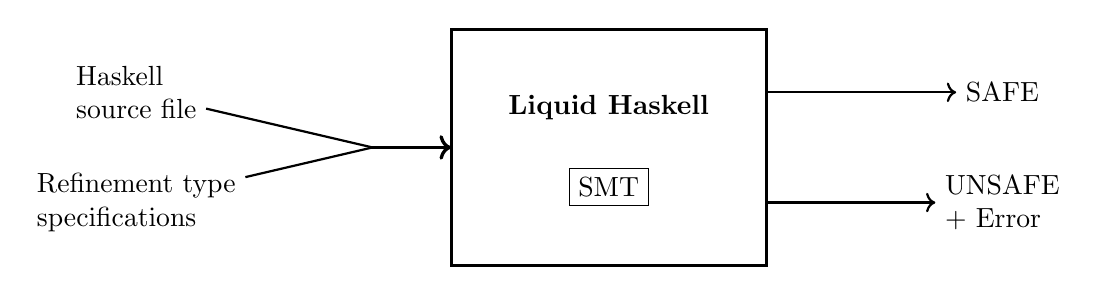
\begin{tikzpicture}
\draw[black, very thick] (3,0) rectangle (7,3);
\node[align=left] (0) at (5,2) {\textbf{Liquid Haskell}};
\node[align=left] (1) at (-1,2.2) {Haskell\\source file};
\node[align=left] (2) at (-1,0.8) {Refinement type\\specifications};
\node[align=left] (3) at (10,2.2) {SAFE};
\node[align=left] (4) at (10,0.8) {UNSAFE\\+ Error};
\node[draw, align=left] (5) at (5,1) {SMT};

\draw[thick] (1) -- (2,1.5);
\draw[thick] (2) -- (2,1.5);
\draw[->,very thick] (2,1.5) -- (3,1.5);

\draw[->,thick] (7,2.2) -- (3);
\draw[->,thick] (7,0.8) -- (4);
\end{tikzpicture}
\caption{Liquid Haskell (simplified).}
\label{fig:LH}
\end{figure}

Liquid Haskell allows us to specify precise properties and invariants about our Haskell code. Those properties can be used intuitively in the refinement type as shown in \Cref{fig:introex}. Here, we define the refinement type \textbf{Even} in Line 1. It says that an integer is even iff it is divisible by two without remainder. Then we can set a number, for example six, that is of this type. Without the Liquid Haskell refinement in Line 3, it would also be allowed to set an odd number as \texttt{evenNumber}, which is obviously not intended in this case. Hence, Liquid Haskell protects us from making a mistake. 
The advantage of setting a refinement type is that desired properties of the functions are visible directly in their signatures and automatically checked by Liquid Haskell.

\begin{figure}[h]
\begin{lstlisting}[mathescape=true, language=haskell, caption={Refinement Example.},captionpos=b, label=fig:introex]
$\LHl$ type $\textbf{Even}$ = {v:Int | v mod 2 $==$ 0} $\LHr$

$\LHl$ $\texttt{evenNumber}$ :: $\textbf{Even}$ $\LHr$
$\texttt{evenNumber}$ :: Int
$\texttt{evenNumber}$ = 6
\end{lstlisting}
\end{figure}

Since binomial and Fibonacci heaps have good amortized bounds, which are constant or logarithmic, we also want to automatically prove them within our program. Hence the second goal of this thesis is then to perform an amortized cost analysis of the formalized data structures. For this purpose, we again use Liquid Haskell with an additional library that allows us to keep track of costs. This enables us to perform the analysis directly within the refinement type. Moreover, we formalized that for a binomial heap, the amortized cost is bound not only by the number of binomial trees it contains but also by the logarithm of the number of its nodes.



\paragraph{Overview.} The subsequent chapters of this thesis are structured as follows: Chapter \ref{sec:related} discusses related work, while Chapters \ref{prel_binomial} and \ref{prel_fibonacci} respectively introduce the preliminaries of binomial and Fibonacci heaps including their functions. Chapter \ref{sec:amortized} outlines the fundamentals of amortized cost analysis, and we apply the analysis to our data structures on paper. In the next chapter, we focus on Liquid Haskell, explaining the workflow, refinement types, proofs, program efficiency, and formalizing binomial and Fibonacci heaps within the program. Finally, we provide a formalization of an amortized analysis of both data structures in Chapter \ref{sec:formalization} and conclude with potential future work in Chapter \ref{sec:conclusion}.



\chapter{Related Work}\label{sec:related}
%Niki Red-Black Trees
%Niki Ticks
%Was mache ich anders/besser?
%Comparison section

Certainly, formalizing binomial and Fibonacci heaps is not a novel endeavor. Previous literature has explored these data structures or attempted to provide amortized cost analyses on paper \cite{brodal2012strict,thomas2022,skew2020,okasaki1999,sadagopanFib,thesis2019stuewe, tarjan1985amortized}. Notably, Daniel Stüwe's master's thesis \cite{thesis2019stuewe} delves into the verification of Fibonacci heaps in Imperative HOL, while Simon Griebel's master's thesis \cite{thesis2019griebel} builds upon Stüwe's work by focusing on the decrease-key operation of Fibonacci heaps. However, there are significant distinctions between these prior works and the present thesis, which we outline in this short chapter. There also exists prior work on refining invariants of data structures such as Red-Black trees \cite{vazou2014liquidhaskell} or analyzing (non-amortized) costs in Liquid Haskell \cite{handley2019liquidate}. However, in this thesis, we provide an amortized cost analysis for two data structures within Liquid Haskell while also refining required invariants. Additionally, we discovered an existing Liquid Haskell implementation of binomial heaps \cite{skew2020}. In this chapter, we will clarify the rationale behind providing another implementation of binomial heaps.

We start by highlighting the differences in the formalization of Fibonacci heaps. Stüwe's formalization places a strong emphasis on proving invariants and correctness properties of Fibonacci heaps. In contrast, my formalization mainly focuses on the amortized cost analysis of the data structure, aiming to set as few properties as needed. Stüwe employs Isabelle HOL, a formal proof assistant, for the formalization and verification of Fibonacci heaps, whereas I utilize Liquid Haskell, which can be applied to an existing implementation of the programming language Haskell. Unlike proving the amortized cost of the functions separately in lemmas, we can directly declare it in the refinements of Liquid Haskell. Refining the types of the function can be useful while programming to directly check if the implemented function indeed returns the desired output.
One aspect missing in Stüwe's thesis, which he also mentions in his outlook chapter, is a formalization of the decrease-key and delete functions. This is addressed in Griebel's master's thesis. Griebel verifies the delete-key operation of Fibonacci heaps in Imperative HOL. However, Griebel employs a different approach than Stüwe, making it a separate formalization rather than a direct extension of Stüwe's work.

The original implementation of binomial heaps by Paul Palmer was developed using Liquid Haskell Version 0.8.6.2. However, this version of the program is incompatible with the newer version of Liquid Haskell (0.9.2.5) that we are using. When attempting to run Palmer's program, we encounter unbound symbol errors in the refinement. This is because in the newer version, refinement types cannot be set in the same manner. For example, the refinement types used in Palmer's version cannot access the outer type within the inner one, as shown below:
\begin{lstlisting}[mathescape=true, language=haskell]
$ts$:[{$t$:$\textbf{Tree a}$ | $\texttt{length}$ $ts$ > rank $t$}].
\end{lstlisting}

To express the desired property within the new Liquid Haskell version, the refinements would have to be completely renewed. Instead of rewriting all those refinements in Palmer's version, there exists the \{-$@$ LIQUID \texttt{"-\;-\;bscope"} $@$-\} flag which eliminates this refinement problem. However, even when solving the unbound symbol errors, other issues still persist. The online Liquid Haskell demo\footnote{http://goto.ucsd.edu:8090/index.html\#?demo=permalink\%2F1675311619\_18955.hs} uses version 0.8.6.0, where Palmer's program compiles and is verified as safe.

Moreover, Palmer's implementation relies on the Liquid.Bag library, which in turn depends on Data.Map. If we aim to prove that those imported operators have certain properties, we would need to reimplement them in order to state them in the refinement. Additionally, Palmer works with tree lists, necessitating the conversion of heaps to tree lists and lists to heaps in all heap functions. In contrast, we view a heap as a type that is exactly a list of binomial trees with some refinement. Due to these complexities, conducting an amortized cost analysis would be very complex in Palmer's version. Therefore, we decided to formalize binomial heaps in a simpler manner rather than extending the existing code.

%Stüwe: proves Invariants and correctness, uses Isabelle HOL, has also imperative implementation which is too complex to be extended (according to Gribel), Hoare Logic for amortized time, another implementation with multiple priority keys.
%No decrease key, no delete function
%definition fib-log’ :: "nat ⇒ nat" where
%"fib-log’ n = nat dext-log ((1 + sqrt 5) / 2) ne + 3"
%definition pop-min-time :: "nat ⇒ nat" where
%"pop-min-time n = 105 + fib-log’ n · 95"

%Griebel: heap is modeled as a map from addresses to (abstract) heap nodes, is not a direct extention of Stüwe because the two approaches are different; no heap-insert, delete-min functions, NO amortization


\chapter{Introduction to Binomial Heaps}\label{prel_binomial}
Binomial heaps are composed of binomial trees and therefore a separate explanation of them is required. This chapter initiates the definition of binomial trees in Section \ref{sec:bitree} by highlighting key properties. Subsequently, attention is directed towards binomial heaps, encompassing their representation in Section \ref{sec:biheap} and operational functions in Section \ref{bi_fun}.

\section{Binomial Tree}\label{sec:bitree}
\definition{ \textit{Binomial trees}, as delineated by Okasaki \cite{okasaki1999}, are recursively defined as follows: %okasaki
\begin{itemize}
	\item A binomial tree of rank 0 is a singleton node.
	\item A binomial tree of rank $r$ + 1 is formed by linking two binomial trees of rank $r$, making one tree the leftmost child of the other.
\end{itemize}
}
An illustration of binomial trees is provided in Figure \ref{fig:bin}.
We adopted Okasaki's definition of binomial trees \cite{okasaki1999} as the foundation for our functional implementation. Through this definition, several properties of binomial trees can be derived.
However, for certain properties not explicitly defined by Okasaki \cite{okasaki1999} but outlined in Lemma \ref{lem_bitree} and Corollary \ref{cor_bitree}, we refer to Cormen et al. \cite{thomas2022}. We include the proofs of these properties in this thesis for clarity and completeness.

\definition{The \textit{height} of a node $p$ in a tree is the number of edges on the longest path from the node to a leaf. If $p$ is a leaf, then the height of $p$ is 0 \cite{goodrich2014data}.
}
\definition{The \textit{depth} of a node $p$ in a tree is the number of edges from the node to the tree's root node. If $p$ is a root node, then the depth of $p$ is 0 \cite{goodrich2014data}.
}

Note that the rank of the root node corresponds to the height of the tree and that height and depth of a tree are equal.

\lemma\label{lem_bitree}{For a binomial tree $B_k$ %Thomas
\begin{enumerate}
	\item there are $2^k$ nodes,
	\item the rank of the tree is $k$,
	\item there are exactly $k \choose i$ nodes at depth $i$ for $i = 0, 1,\dots ,k$, and
	\item the root has rank $k$, which is greater than that of any other node; moreover if
	the children of the root are numbered from left to right by $k-1, k-2, \dots, 0$,
	child $i$ is the root of a subtree $B_i$.
\end{enumerate}}

\begin{figure}[h]
	\centering
	\begin{subfigure}[t]{.2\textwidth}
		\centering
		Rank 0 \par\medskip
		
\begin{tikzpicture}
			[every node/.style={fill,circle,inner sep=1pt}]
			Rank 0
			\node {a};
		\end{tikzpicture}
	\end{subfigure}	
	\begin{subfigure}[t]{.2\textwidth}
		\centering
		Rank 1 \par\medskip	
		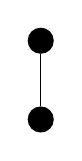
\begin{tikzpicture}
			[level distance=10mm,
			every node/.style={fill,circle,inner sep=1pt}]
			\node {a}
			child {node {a}};
		\end{tikzpicture}
	\end{subfigure}
	\begin{subfigure}[t]{.2\textwidth}
		\centering
		Rank 2 \par\medskip	
		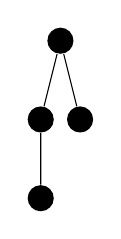
\begin{tikzpicture}
			[level distance=10mm,
			every node/.style={fill,circle,inner sep=1pt},
			level 1/.style={sibling distance=5mm}]
			\node {a}
			child {node {a}
				child {node {a}}
			}
			child {node {a}};
		\end{tikzpicture}
	\end{subfigure}
	\begin{subfigure}[t]{.2\textwidth}
		\centering
		Rank 3 \par\medskip	
		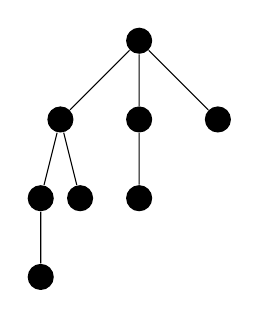
\begin{tikzpicture}
			[level distance=10mm,
			every node/.style={fill,circle,inner sep=1pt},
			level 1/.style={sibling distance=10mm},
			level 2/.style={sibling distance=5mm}]
			\node {a}
			child {node {a}
				child {node {a}
					child {node {a}}
				}
				child {node {a}}
			}
			child {node {a}
				child {node {a}
					child[missing]
				}	
			}
			child {node {a}};
		\end{tikzpicture}
	\end{subfigure}
	
	\begin{subfigure}[t]{0.6\textwidth}
		\centering
		\quad \qquad Rank 4 \par\medskip	
		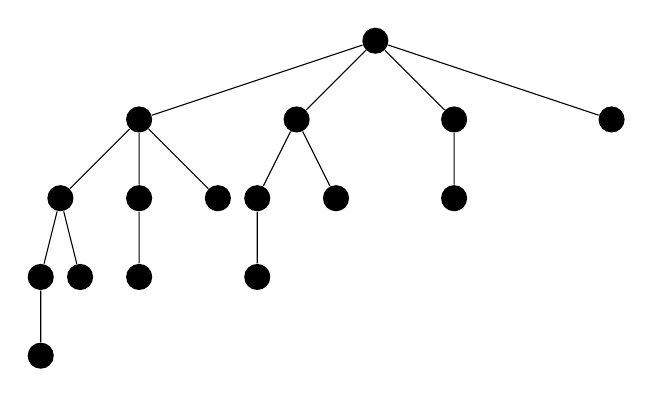
\begin{tikzpicture}
			[level distance=10mm,
			every node/.style={fill,circle,inner sep=1pt},
			level 1/.style={sibling distance=20mm},
			level 2/.style={sibling distance=10mm},
			level 3/.style={sibling distance=5mm}]
			\node {a}
			child {node {a}
				child {node {a}
					child {node {a}
						child {node {a}}
					}
					child {node {a}}
				}
				child {node {a}
					child {node {a}
						child[missing]
					}	
				}
				child {node {a}}
			}
			child {node {a}
				child {node {a}
					child {node {a}}
				}
				child {node {a}}
			}
			child {node {a}
				child {node {a}}
			}
			child {node {a}};
		\end{tikzpicture}
	\end{subfigure}
	\caption{Binomial trees of ranks $0 - 4$.}
	\label{fig:bin}
\end{figure}
%Thomas
\proof{The proof is by induction on $k$. To establish each property, we begin with the base case of the binomial tree $B_0$. Confirming the validity of each property for $B_0$ is straightforward.
	For the inductive step, we assume that the lemma holds for $B_{k-1}$.
\begin{enumerate}
	\item The binomial tree $B_k$ is formed by combining two copies of $B_{k-1}$, resulting in a total of $2^{k-1} + 2^{k-1} = 2^k$ nodes.
	\item Due to the way in which the two instances of $B_{k-1}$ are linked to create $B_k$, the
	rank of a node in $B_k$ exceeds that of $B_{k-1}$ by one.
	According to the inductive hypothesis, this increased rank equals $(k - 1) + 1 = k$.
	\item Let $D(k,i)$ represent the number of nodes at depth $i$ of the binomial tree $B_k$. Since $B_k$
	consists of two copies of $B_{k-1}$ linked together, nodes at depth $i$ in $B_{k}$
	compose of the nodes of $B_{k-1}$ at depth $i$ and the nodes at depth $i - 1$ of the appended tree $B_{k-1}$. Thus,
	\begin{align*}
		D(k,i) &= D(k-1,i) + D(k-1,i-1) \\
		&= {k-1 \choose i} + {k-1 \choose i-1} = {k \choose i}.
	\end{align*}
	\item The only node with a higher rank in $B_k$ than in $B_{k-1}$ is the root, which
	gains one more child compared to $B_{k-1}$. Since the root of $B_{k-1}$ has rank $k-1$,
	the root of $B_k$ has rank $k$. Furthermore, based on the inductive hypothesis, the children of the root of $B_{k-1}$ are roots of $B_{k-2},B_{k-3},\dots,B_0$, arranged from left to right. Consequently, when $B_{k-1}$ is linked to $B_{k-1}$, the children of the root of the resulting tree are roots of $B_{k-1},B_{k-2},B_{k-3},\dots,B_0$.
\end{enumerate}\qed
}
%Thomas
\corollary\label{cor_bitree}{The maximum rank of any node in an $n$-node binomial tree is $\log_2(n)$.}
\proof{This proof is deduced from properties 1 and 4 of Lemma \ref{lem_bitree}. Since the root contains the maximum rank $k$ and there are $2^k$ nodes in the tree, we conclude
\[   k = \log_2(2^k)=\log_2(n) .\] \qed}

The term \enquote{binomial tree} derives its name from property 3 of Lemma \ref{lem_bitree} because the expression $k \choose i$ is the binomial coefficient.

\section{Binomial Heap}\label{sec:biheap}
A binomial heap consists of heap-ordered binomial trees, each with a distinct rank, and the collection is represented as a list of trees arranged in ascending order based on their ranks \cite{okasaki1999}.
Again we refer to the properties presented by Cormen et al. \cite{thomas2022} that define a binomial heap as in Definition \ref{bin_def}.
\definition{\label{bin_def}A \textit{binomial heap} $H$ is a set of binomial trees that satisfies the following properties: %Thomas
	\begin{itemize}
		\item Each node has a key.
		\item Each binomial tree in $H$ obeys the min-heap property: the key of a node is
		greater than or equal to the key of its parent. We say that each such a tree is
		\textit{min-heap-ordered}.
		\item For any non-negative integer $k$, there is at most one binomial tree in $H$ whose
		root has rank $k$.
	\end{itemize}
 }

The trees in a binomial heap of size $n$ correspond to the binary representation of $n$. This is because each tree $B$ in a binomial heap has a unique rank $k$ and $B_k$ has $2^k$ nodes \cite{okasaki1999}.

\example{Consider a binomial heap with 22 nodes, whose binary representation is $10110$. This heap would contain one tree each with 2 nodes, 4 nodes and 16 nodes. The trees have rank 1, 2, and 4 corresponding to the position of the ones in the binary representation.}


\section{Functions of Binomial Heaps}\label{bi_fun}
The implementation of the basic functions of binomial heaps in this thesis is based on Okasaki's book \cite{okasaki1999}. These functions are \texttt{insert}, \texttt{merge}, \texttt{findMin} and \texttt{deleteMin}. In addition to explaining the functions, we already provide some Liquid Haskell code. This code looks similar to the known Haskell type system but extends it with refinements and is hence more expressive. Moreover, the Liquid Haskell code directly states intuitive properties of data structures and functions which helps to understand the code. The more rigorously we refine our data structure, the easier it becomes to prove further properties.

\begin{figure}[h]
\begin{lstlisting}[mathescape=true, language=haskell, caption={Refinement of the data structure \textbf{BiTree a}.},captionpos=b, label=fig:Bitree]
data $\textbf{BiTree a}$ =   
   Node 
	{ rank :: $\textbf{Nat}$
	, root :: $\textbf{a}$
	, subtrees :: {$s$:[$\textbf{BiTree a}$] | rank $==$ length $s$ && 
		(length $s$ $==$ 0 || length $s$ > 0 && 
		rank $==$ $\texttt{getRank}$ (head $s$) + 1) && $\texttt{sorted}$ root $s$ 
		&& $\texttt{ordRank}$ $s$}
	}
\end{lstlisting}
\end{figure}

Before moving on to implementing a binomial heap, which consists of a list of binomial trees, we first need to formalize binomial trees. A node in a binomial tree stores its rank, its root element and a list of its children. While the rank is simply a natural number and the root is an element of type \textbf{a}, the refinement type of the children is more complex. This is because we not only want the subtrees to be a list of binomial trees but also to ensure a descending order of ranks. Moreover, we require that the list is exactly as long as the rank of the node and that every child has a rank smaller than the rank of its parent. Additionally, we want the list to be ordered by rank and the tree to be sorted. All those properties which are the intuitive definition of the data structure can be expressed in the refinement as illustrated in \Cref{fig:Bitree}.

In this code snippet we specify that the rank is a natural number instead of just an integer. For the subtrees, the constraint \enquote{\lstinline{rank == length} $s$} ensures that the length of the child list $s$ is exactly as long as the rank of the node. To assert that the ranks of the children are smaller than that of their parent, we specify that the rank of the first element of the list is exactly one less than the node's rank. Because we need to access the first element of the list, we differentiate between the empty list and a list of length greater than zero. Additionally, \texttt{\lstinline{ordRank}} is a separate function that ensures the ranks of the subtrees are ordered in the list. More concisely, \texttt{\lstinline{ordRank}} checks if the rank of each element is exactly one less than the rank of the previous element. The refinement \texttt{\lstinline{sorted}} takes the root element and the subtree list as an input and verifies that the root element is smaller than every other element of the list.
\FloatBarrier
As a next step, we define the type of a binomial heap in our code, as shown in \Cref{fig:Biheap}. Here, a binomial heap is simply a list of binomial trees that fulfills a property \texttt{\lstinline{ordRankH}}. This function is similar to the \texttt{\lstinline{ordRank}} function, but instead of requiring a rank decrease of exactly one, it simply requires the ranks of the list to be increasing. We will see the connection of \texttt{\lstinline{ordRankH}} and \texttt{\lstinline{ordRank}} in Lemma \ref{lem:oRtoORH} in a later chapter.

\begin{figure}[h]
\begin{lstlisting}[mathescape=true, language=haskell, caption={Refinement of the data structure \textbf{BiHeap a}.},captionpos=b, label=fig:Biheap]
	  type $\textbf{BiHeap a}$ = {$ts$:[$\textbf{BiTree a}$] | $\texttt{ordRankH}$ $ts$}
\end{lstlisting}
\end{figure}

After defining our heap, we proceed with the heap functions. The implementation of \texttt{insert} is presented in \Cref{fig:Binsert}. 
To insert a new element $x$ into the heap we initially create a singleton. A singleton is merely a node with rank zero, the root element $x$ and a empty list of children. Then, we traverse the list and compare the ranks, which is accomplished in the helper function $\texttt{insTree}$. It's important to note that the rank cannot exceed that of the compared tree because we always insert a node with rank zero. If the rank is lower than that of the compared tree, we insert the node at this point in the tree list. If two trees have equal ranks, we link them together using the $\texttt{link}$ function, and then continue inserting the linked tree. For linking, we simply attach the node with the larger root element under the node with the smaller element.
In Section \ref{amortized_bin1} we demonstrate that $\texttt{insert}$ runs in constant amortized time.

\begin{figure}[h]
\begin{lstlisting}[mathescape=true, language=haskell,caption={Insert function.},captionpos=b, label=fig:Binsert]
$\texttt{link}$ $t_1$@(Node r $x_1$ $ts_1$) $t_2$@(Node _ $x_2$ $ts_2$) =
	| $x_1 \leq x_2$ = Node ($r + 1$) $x_1$ ($t_2$:$ts_1$)
	| otherwise = Node ($r + 1$) $x_2$ ($t_1$:$ts_2$)
	
$\texttt{insTree}$ $t$ [] = [$t$]
$\texttt{insTree}$ $t$ $ts$@($t'$:$ts'$) 
	| rank $t$ < rank $t'$ = $t$ : $ts$
	| otherwise = $\texttt{insTree}$ ($\texttt{link}$ $t$ $t'$) $ts'$

$\texttt{insert}$ $x$ $ts$ = $\texttt{insTree}$ (Node $0$ $x$ []) $ts$
\end{lstlisting}
\end{figure}

The function $\texttt{merge}$ combines two heaps, and whenever two trees in the heap have the same rank, they are linked and inserted into the merged heap. This procedure is illustrated in \Cref{fig:Bmerge}.

\begin{figure}[h]
\begin{lstlisting}[mathescape=true, language=haskell, caption={Merge function.},captionpos=b, label=fig:Bmerge, abovecaptionskip=\bigskipamount]
$\texttt{merge}$ $ts_1$ [] = $ts_1$
$\texttt{merge}$ [] $ts_2$ = $ts_2$
$\texttt{merge}$ $ts_1$@($t_1$:$ts_1'$) $ts_2$@($t_2$:$ts_2'$)
	| rank $t_1$ $<$ rank $t_2$ = $t_1$ : $\texttt{merge}$ $ts_1'$ $ts_2$
	| rank $t_2$ $<$ rank $t_1$ = $t_2$ : $\texttt{merge}$ $ts_1$ $ts_2'$
	| otherwise = $\texttt{insTree}$ ($\texttt{link}$ $t_1$ $t_2$) ($\texttt{merge}$ $ts_1'$ $ts_2'$)
\end{lstlisting}
\end{figure}

To locate and remove the minimum element of the heap, we define a helper function called \texttt{removeMinTree}, which returns a tuple. The first element of the tuple is the tree whose root is the minimum element, and the second element contains the list of remaining trees in the heap without the extracted tree. When deleting the minimum element, we just call \texttt{removeMinTree} that extracts the tree with the minimum element in the root and subsequently merge its children with the remaining heap. Additionally, we utilize the Prelude Haskell function \texttt{reverse} in \texttt{deleteMin} to obtain a heap with an increasing order of ranks. We illustrate the functions in \Cref{fig:Bdelete}. In those functions we do not consider an empty heap, because in that case we cannot find or delete anything.

\begin{figure}[h]
\begin{lstlisting}[mathescape=true, language=haskell, caption={Find and delete minimum functions.},captionpos=b, label=fig:Bdelete ]
$\texttt{removeMinTree}$ [$t$] = ($t$,[])
$\texttt{removeMinTree}$ ($t$:$ts$) = 
	let ($t'$, $ts'$) = $\texttt{removeMinTree}$ $ts$ in
	if root $t$ $<$ root $t'$ then ($t$, $ts$) else ($t'$, $t$:$ts'$)
	
$\texttt{findMin}$ $ts$ = let ($t$,_) = $\texttt{removeMinTree}$ $ts$ in root $t$

$\texttt{deleteMin}$ $ts$ = let (Node _ $x$ $ts_1$, $ts_2$) = $\texttt{removeMinTree}$ $ts$ in
	$\texttt{merge}$ ($\texttt{reverse}$ $ts_1$) $ts_2$
\end{lstlisting}
\end{figure}

All explained functions of binomial heaps run at worst in $O(\log_2 n)$ time \cite{okasaki1999}. 

\chapter{Introduction to Fibonacci Heaps}\label{prel_fibonacci}
The Fibonacci heap data structure is designed to serve as both a mergeable heap and to support operations with constant amortized time. A mergeable heap is according to Cormen et al. \cite{thomas2022} any data structure that supports the five operations: \texttt{makeHeap}, \texttt{insert}, \texttt{findMin}, \texttt{extractMin} and \texttt{merge}. Further, we will discuss an amortized analysis in Section \ref{sec:amortized}. Operations such as \texttt{insert}, \texttt{extractMin}, and \texttt{decreaseKey} run efficiently in Fibonacci heaps, making them suitable for applications that involve frequent invocations of these operations. 

\section{Fibonacci Heap}
\definition{A \textit{Fibonacci heap} is a collection of rooted trees that are min-heap ordered. That is, each tree obeys the min-heap property: the key of a node is greater than or equal to the key of its parent \cite{thomas2022}.}

\begin{figure}[h]
	\centering
	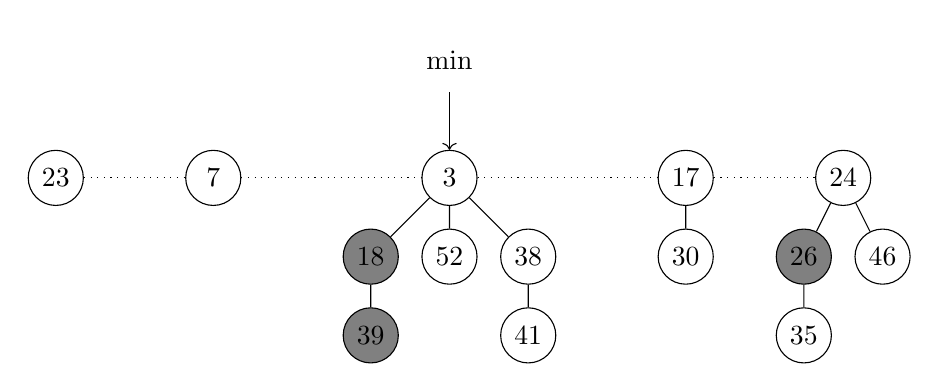
\begin{tikzpicture}
	[level distance=10mm,
	every node/.style={circle,draw,inner sep=2pt,minimum size=.7cm},
	level 1/.style={sibling distance=10mm},
	level 2/.style={sibling distance=5mm}]
	\node (23) at (0,0) {23};
	\node (7) at (2,0) {7};
	\node (min) [draw=none] at (5,1.5) {min};
	\node (3) at (5,0) {3}
	child {node [fill=gray]  {18}
		child {node [fill=gray]  {39}}
	}
	child {node {52}}
	child {node {38}
		child {node {41}
		}	
	};
	\node (17) at (8,0) {17}
	child {node {30}
	};
	\node (24) at (10,0) {24}
	child {node [fill=gray] {26}
		child {node {35}}
	}
	child {node {46}	
	};
	\draw [dotted] (23) -- (7) -- (3) -- (17) -- (24);
	\draw [->] (min) -- (3);
	\end{tikzpicture}	
	\caption{Fibonacci heap \cite{thomas2022}.}
	\label{fig:exfib}
\end{figure}

We avoid imposing explicit constraints on the number or structure of these trees, instead, constraints are implicit in the manipulation of the trees \cite{fredman1987fibonacci}. The construction of a Fibonacci heap and the operations performed on it will be explained in Section \ref{fib_fun}. 

Figure \ref{fig:exfib} provides an example of a Fibonacci heap. In this instance, the heap comprises a total of fourteen nodes and consists of five min-heap-ordered trees. The dotted line delineates the root list of the heap and the minimum element of the heap, indicated by an arrow, is the number three. Nodes colored in grey are marked nodes, whereas all others are unmarked.

In a non-functional implementation, the data structure is often represented with each node containing pointers to its parent and a pointer to any of its children \cite{brodal2012strict, kaplan2014fibonacci, fredman1987fibonacci}. Additionally, the children are typically linked together in a circular, doubly linked list \cite{thomas2022, fredman1987fibonacci}. However, Haskell does not support access via pointers, which is why we implemented Fibonacci heaps in an abstract manner. This implementation is outlined in Section \ref{fib_fun}.

\section{Functions of Fibonacci Heaps}\label{fib_fun}
In this section, we provide a more concrete representation of Fibonacci heaps by demonstrating the implementation of the heap functions. We begin by defining the data structure in \Cref{fig:fibheap}. To achieve this, we first define a Fibonacci tree in \Cref{fig:fibtree}, where each node consists of a depth, a root element, a list of its subtrees, and an indication of whether it is marked or not. We refine the depth to be positive. Moreover, the function \texttt{equalDepth} indicates that all siblings have the same depth. Additionally, we require that the depth of a parent is exactly one smaller than the depth of its children. We will need this constraint for a termination proof, where depth serves as a termination metric. Termination and totality is necessary such that modeled proofs by induction on recursive functions are sound. Hence Liquid Haskell provides a powerful termination and totality checker and rejects any definition that it cannot prove to be terminating and total \cite{vazou2018theorem}. To access the first element of the list, we need to differentiate between an empty list and a list that contains at least one element.

\begin{figure}[h]
\begin{lstlisting}[mathescape=true, language=haskell, caption={Refinement of the data structure \textbf{FibTree a}.},captionpos=b, label=fig:fibtree]
data $\textbf{FibTree a}$ = 
   Node 
	{ depth :: $\textbf{Pos}$
	, root :: $\textbf{a}$
	, subtrees :: {$s$:[$\textbf{FibTree a}$] | length $s$ $==$ 0 || 
		($\texttt{equalDepth}$ $s$ && $\texttt{getDepth}$ (head $s$) $==$ depth + 1)}
	, marked :: Bool
	}
\end{lstlisting}
\end{figure}

A Fibonacci heap, as defined in \Cref{fig:fibheap}, is either empty or composed of two components: \lstinline{minTree} and \lstinline{trees}. The \lstinline{trees} component is a list of trees contained in the heap, excluding \lstinline{minTree}. Here, \lstinline{minTree} refers to a tree that has the minimum element of the heap as its root, and we will henceforth denote it as the \emph{minimum tree}. Maintaining a record of marked nodes in Fibonacci trees is crucial for the amortized cost analysis of the heap.

\begin{figure}[h]
\begin{lstlisting}[mathescape=true, language=haskell, caption={Refinement of the data structure \textbf{FibHeap a}.},captionpos=b, label=fig:fibheap]
data $\textbf{FibHeap a}$ = E | FH { minTree :: $\textbf{FibTree a}$
			, trees :: [$\textbf{FibTree a}$]}	
\end{lstlisting}
\end{figure}

Once again, we have fundamental operations such as \texttt{insert}, \texttt{merge}, \texttt{findMin}, and \texttt{deleteMin}.
As the name indicates, the \texttt{insert} function inserts an element $x$ into a given heap. In contrast to the \texttt{insert} function of binomial heaps, here, we do not need to link trees with the same degree because we allow multiple trees of the same degree. Therefore, our focus is on ensuring that the tree with the minimum element is separated from the rest of the tree list. This separation happens in the \texttt{merge} function, which compares the minimum elements of two heaps and selects the tree with the smaller one to be the \lstinline{minTree} of the newly created Fibonacci heap. Subsequently, \texttt{insert} merges a singleton containing the element $x$ with the current heap. In this scenario, a singleton refers to a Fibonacci heap that solely consists of one unmarked node with the element $x$. \Cref{fig:Fcode1} illustrates the functions \texttt{singleton}, \texttt{merge} and \texttt{insert}.

\begin{figure}[h]
\begin{lstlisting}[mathescape=true, language=haskell, caption={Singleton, merge and insert functions.},captionpos=b, label=fig:Fcode1]
$\texttt{singleton}$ $x$ = FH (Node 1 $x$ [] False) []

$\texttt{merge}$ E $h$ = $h$
$\texttt{merge}$ $h_1$@(FH $minTr_1$ $ts_1$) $h_2$@(FH $minTr_2$ $ts_2$)
     | root $minTr_1$ $<$ root $minTr_2$ = 
     	FH $minTr_1$ ($minTr_2$ : $ts_2$ ++ $ts_1$)
     | otherwise = 
     	FH $minTr_2$ ($minTr_1$ : $ts_1$ ++ $ts_2$)

$\texttt{insert}$ $h$ $x$ = $\texttt{merge}$ $h$ ($\texttt{singleton}$ $x$)
\end{lstlisting}
\end{figure}

Figure \ref{fig:Finsert} shows a Fibonacci heap where the element 21 is inserted in the Fibonacci heap depicted in Figure \ref{fig:exfib}. The newly inserted node is highlighted in red. Since 21 is greater than the current minimum element, which is the number three, we do not alter the minimum tree and simply append the node to the root list. In general, the arrangement of the trees is not important in this data structure. However, due to the similarities to binomial heaps, we chose to implement it as a list.

\begin{figure}[h]
	\centering
	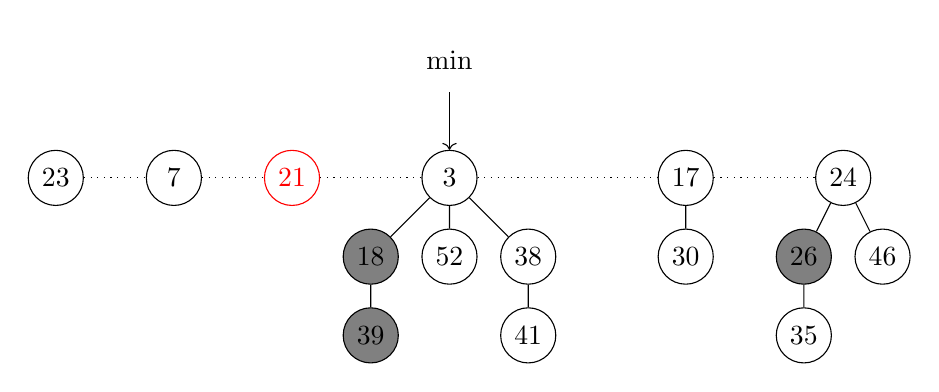
\begin{tikzpicture}
	[level distance=10mm,
	every node/.style={circle,draw,inner sep=2pt,minimum size=.7cm},
	level 1/.style={sibling distance=10mm},
	level 2/.style={sibling distance=5mm}]
	\node (23) at (0,0) {23};
	\node (7) at (1.5,0) {7};
	\node (21) [red] at (3,0) {21};
	\node (min) [draw=none] at (5,1.5) {min};
	\node (3) at (5,0) {3}
	child {node [fill=gray]  {18}
		child {node [fill=gray]  {39}}
	}
	child {node {52}}
	child {node {38}
		child {node {41}
		}	
	};
	\node (17) at (8,0) {17}
	child {node {30}
	};
	\node (24) at (10,0) {24}
	child {node [fill=gray] {26}
		child {node {35}}
	}
	child {node {46}	
	};
	\draw [dotted] (23) -- (7) -- (21) -- (3) -- (17) -- (24);
	\draw [->] (min) -- (3);
	\end{tikzpicture}	
	\caption{Inserting a node \cite{thomas2022}.}
	\label{fig:Finsert}
\end{figure}
\FloatBarrier
Finding the minimum element in the heap is straightforward due to the representation of the Fibonacci heap. The minimum element is simply the root element of the separated minimum tree.

\begin{figure}[h]
\begin{lstlisting}[mathescape=true, language=haskell, caption={Finding the minimum element.},captionpos=b]
$\texttt{findMin}$  = root . minTree
\end{lstlisting}
\end{figure}

Deleting the minimum element of the heap is more complex. This function involves postponed work of consolidating trees in the root list. Initially, when we remove the minimum element, which is the root of \lstinline{minTree}, we add all of its subtrees to the tree list. The subsequent step involves attempting to reduce the length of the tree list by linking trees of the same degree. Finally, we need to extract the new minimum tree that includes the minimum element. To execute these steps, we utilize the auxiliary functions \texttt{extractMin}, \texttt{consolidate}, \texttt{meld}, and \texttt{link} that are illustrated in \Cref{fig:Fcode2}. The \texttt{extractMin} function traverses the list of Fibonacci trees and extracts the one with the minimum element. The \texttt{consolidate} function invokes \texttt{meld} with each element, which links trees of the same degree, where the \emph{degree} of a tree denotes number of the root node's children. For calculating the degree of a tree, we use the helper function \texttt{getDegree}. Additionally when linking, it unmarks the node where a tree is attached to.

\begin{figure}[h]
\begin{lstlisting}[mathescape=true, language=haskell, caption={Link, meld, consolidate, extract minimum and delete minimum functions.},captionpos=b, label=fig:Fcode2]
$\texttt{link}$ $t_1$@(Node $d$ $x_1$ $ts_1$ _) $t_2$@(Node _ $x_2$ $ts_2$ _)
	| $x_1$ $\leq$ $x_2$ = Node $d$ $x_1$ ($t_2$:$ts_1$) False
	| otherwise = Node $d$ $x_2$ ($t_1$:$ts_2$) False

$\texttt{meld}$ [] $t$ = [$t$]
$\texttt{meld}$ ($t_1$:$ts_1$) $t$ 
	| $\texttt{getDegree}$ $t_1$ $==$ $\texttt{getDegree}$ $t$ = $\texttt{meld}$ $ts_1$ ($\texttt{link}$ $t$ $t_1$)
	| otherwise = $t_1$ : $\texttt{meld}$ $ts_1$ $t$

$\texttt{consolidate}$ [$t$] = [$t$]
$\texttt{consolidate}$ ($t$:$ts$) = foldl $\texttt{meld}$ [$t$] $ts$

$\texttt{extractMin}$ [$t$] = ($t$, [])
$\texttt{extractMin}$ ($t$:$ts$)
	| root $t$ < root $t'$ = ($t$, $ts$) 
	| otherwise = (t', t:ts')
	where ($t'$, $ts'$) = $\texttt{extractMin}$ $ts$

$\texttt{deleteMin}$  (FH (Node _ $x$ [] _) []) = E
$\texttt{deleteMin}$  (FH $minTr$ $ts$) = 
	FH $minTr_1$ $ts_1$ where
	($minTr_1$, $ts_1$) = $\texttt{extractMin}$ $\$$ 
		$\texttt{consolidate}$ (subtrees $minTr$ ++ $ts$)
\end{lstlisting}
\end{figure}

We present a step-by-step example of deleting the minimum element of the heap in Figure \ref{fig:Fdelete}. It is important to note that the order of linking may vary depending on the implementation. In this example, we use the Fibonacci heap obtained from the insertion process depicted earlier in Figure \ref{fig:Finsert}. We highlight changes in each step by marking affected nodes in red.
Firstly, we remove the minimum node containing the element three, and add all its three children, that are nodes with elements 18, 52, and 38, to the root list. This step is illustrated in Figure \ref{fig:Fdeleteb}. Next, we link all trees until no trees in the heap have the same degree. Since the nodes with roots 7 and 23 both consist of only one node and hence have degree zero, we make the larger element a child of the smaller one. Consequently, in Figure \ref{fig:Fdeletec}, the node with the element 23 becomes a child of the node with the element 7, resulting in a newly created tree with degree one. In Figure \ref{fig:Fdeleted}, we append the tree with the root 17 to the tree with the root element 7, as both trees are of the same degree. Similar steps are executed in Figures \ref{fig:Fdeletee}, \ref{fig:Fdeletef}, and \ref{fig:Fdeleteg}.
Finally, in Figure \ref{fig:Fdeleteg}, there are only three trees in the heap with different degrees: three, two, and one. The minimum tree is the tree with the root element 7. In this example, deleting the minimum element results in halving the number of trees in the heap.

\begin{figure}[h]
	\centering
	\begin{subfigure}[t]{0.51\textwidth}
		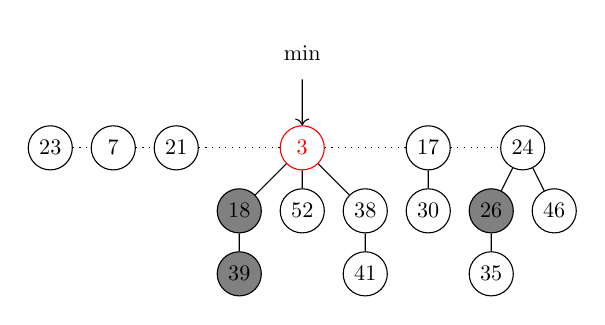
\begin{tikzpicture}
		[scale=0.80, transform shape, level distance=10mm,
		every node/.style={circle,draw,inner sep=2pt,minimum size=.7cm},
		level 1/.style={sibling distance=10mm},
		level 2/.style={sibling distance=5mm}]
		\node (23) at (0,0) {23};
		\node (7) at (1,0) {7};
		\node (21) at (2,0) {21};
		\node (3) [red] at (4,0) {3}
		child {node [fill=gray]  {18}
			child {node [fill=gray]  {39}}
		}
		child {node {52}}
		child {node {38}
			child {node {41}
			}	
		};
		\node (17) at (6,0) {17}
		child {node {30}
		};
		\node (24) at (7.5,0) {24}
		child {node [fill=gray] {26}
			child {node {35}}
		}
		child {node {46}	
		};
		\node (min) [draw=none] at (4,1.5) {min};
		\draw [dotted] (23) -- (7) -- (21) -- (3) -- (17) -- (24);
		\draw [->] (min) -- (3);
	\end{tikzpicture}
	\caption{}
	\label{fig:Fdeletea}
\end{subfigure}
\begin{subfigure}[t]{.49\textwidth}
	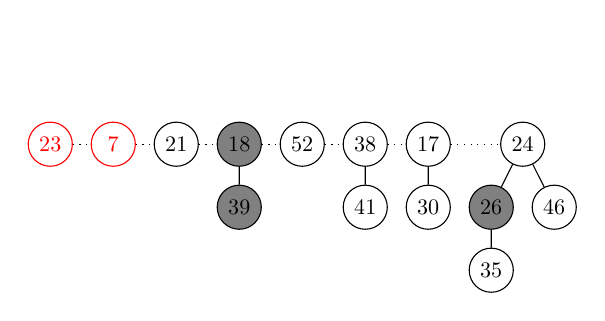
\begin{tikzpicture}
	[scale=0.80, transform shape, level distance=10mm,
	every node/.style={circle,draw,inner sep=2pt,minimum size=.7cm},
	level 1/.style={sibling distance=10mm},
	level 2/.style={sibling distance=5mm}]
	\node (23) [red] at (0,0) {23};
	\node (7) [red] at (1,0) {7};
	\node (21) at (2,0) {21};
	\node (18) [fill=gray] at (3,0) {18}
		child {node [fill=gray]  {39}};
	\node (52) at (4,0) {52};
	\node (38) at (5,0) {38}
		child {node {41}};
	\node (17) at (6,0) {17}
	child {node {30}
	};
	\node (24) at (7.5,0) {24}
	child {node [fill=gray] {26}
		child {node {35}}
	}
	child {node {46}	
	};
	\draw [dotted] (23) -- (7) -- (21) -- (18) -- (52) --(38) -- (17) -- (24);
	\node (min) [draw=none] at (5,1.5) {};
	\end{tikzpicture}\hspace{1cm}%
	\caption{}
	\label{fig:Fdeleteb}
\end{subfigure}
\quad
\begin{subfigure}[t]{.49\textwidth}
	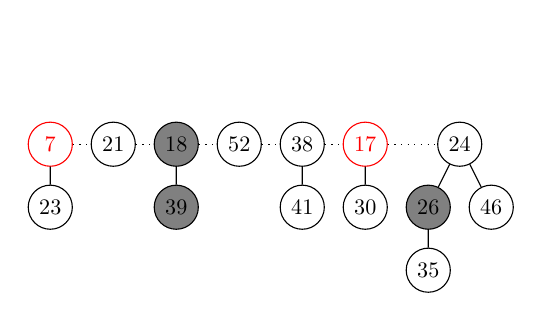
\begin{tikzpicture}
	[scale=0.80, transform shape, level distance=10mm,
	every node/.style={circle,draw,inner sep=2pt,minimum size=.7cm},
	level 1/.style={sibling distance=10mm},
	level 2/.style={sibling distance=5mm}]
	\node (7) [red] at (1,0) {7}
		child {node (23) {23}};
	\node (21) at (2,0) {21};
	\node (18) [fill=gray] at (3,0) {18}
	child {node [fill=gray]  {39}};
	\node (52) at (4,0) {52};
	\node (38) at (5,0) {38}
	child {node {41}};
	\node (17) [red] at (6,0) {17}
	child {node {30}
	};
	\node (24) at (7.5,0) {24}
	child {node [fill=gray] {26}
		child {node {35}}
	}
	child {node {46}	
	};
	\draw [dotted] (7) -- (21) -- (18) -- (52) --(38) -- (17) -- (24);
	\node (min) [draw=none] at (5,1.5) {};
	\end{tikzpicture}\hspace{1cm}%
	\caption{}
	\label{fig:Fdeletec}
\end{subfigure}
%\caption{Deleting the minimum element (a - c) \cite{thomas2022}.}
\begin{subfigure}[t]{.49\textwidth}
	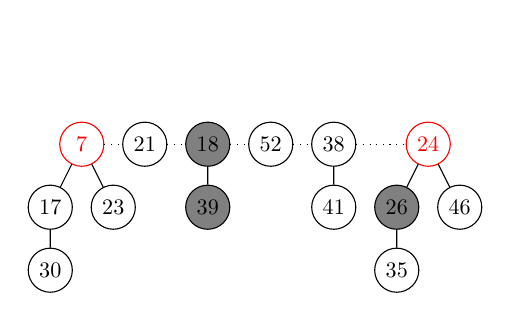
\begin{tikzpicture}
	[scale=0.80, transform shape, level distance=10mm,
	every node/.style={circle,draw,inner sep=2pt,minimum size=.7cm},
	level 1/.style={sibling distance=10mm},
	level 2/.style={sibling distance=5mm}]
	\node (7) [red] at (0,0) {7}
	child {node {17}
	child {node {30}}}
	child {node {23}};
	\node (21) at (1,0) {21};
	\node (18) [fill=gray] at (2,0) {18}
	child {node [fill=gray]  {39}};
	\node (52) at (3,0) {52};
	\node (38) at (4,0) {38}
	child {node {41}};
	\node (24) [red] at (5.5,0) {24}
	child {node [fill=gray] {26}
		child {node {35}}
	}
	child {node {46}	
	};
	\draw [dotted] (7) -- (21) -- (18) -- (52) --(38) -- (24);
	\node (min) [draw=none] at (5,1.5) {};
	\end{tikzpicture}\hspace{1cm}%
	\caption{}
	\label{fig:Fdeleted}
\end{subfigure}
\begin{subfigure}[t]{.49\textwidth}
	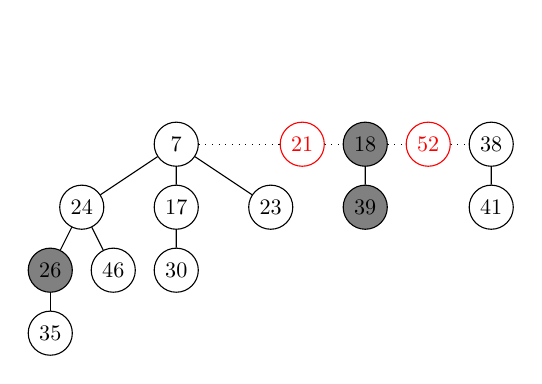
\begin{tikzpicture}
	[scale=0.80, transform shape, level distance=10mm,
	every node/.style={circle,draw,inner sep=2pt,minimum size=.7cm},
	level 1/.style={sibling distance=15mm},
	level 2/.style={sibling distance=10mm}]
	\node (7) at (0,0) {7}
	child {node {24}
	child {node [fill=gray] {26}
		child {node {35}}
	}
	child {node {46}	
	}}
	child {node {17}
		child {node {30}}}
	child {node {23}};
	\node (21) [red] at (2,0) {21};
	\node (18) [fill=gray] at (3,0) {18}
	child {node [fill=gray]  {39}};
	\node (52) [red] at (4,0) {52};
	\node (38) at (5,0) {38}
	child {node {41}};
	\draw [dotted] (7) -- (21) -- (18) -- (52) --(38);
	\node (min) [draw=none] at (5,1.5) {};
	\end{tikzpicture}\hspace{1cm}%
	\caption{}
	\label{fig:Fdeletee}
\end{subfigure}
\begin{subfigure}[t]{.49\textwidth}
	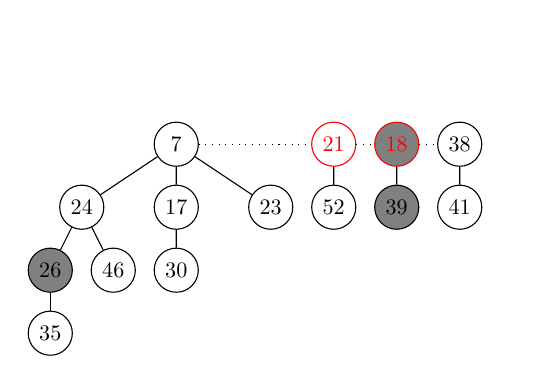
\begin{tikzpicture}
	[scale=0.80, transform shape, level distance=10mm,
	every node/.style={circle,draw,inner sep=2pt,minimum size=.7cm},
	level 1/.style={sibling distance=15mm},
	level 2/.style={sibling distance=10mm}]
	\node (7) at (0,0) {7}
	child {node {24}
		child {node [fill=gray] {26}
			child {node {35}}
		}
		child {node {46}	
	}}
	child {node {17}
		child {node {30}}}
	child {node {23}};
	\node (21) [red] at (2.5,0) {21}
	child {node {52}};
	\node (18) [red,fill=gray] at (3.5,0) {18}
	child {node [fill=gray]  {39}};
	\node (38) at (4.5,0) {38}
	child {node {41}};
	\draw [dotted] (7) -- (21) -- (18) --(38);
	\node (min) [draw=none] at (5,1.5) {};
	\end{tikzpicture}\hspace{1cm}%
	\caption{}
	\label{fig:Fdeletef}
\end{subfigure}
\begin{subfigure}[t]{.49\textwidth}
	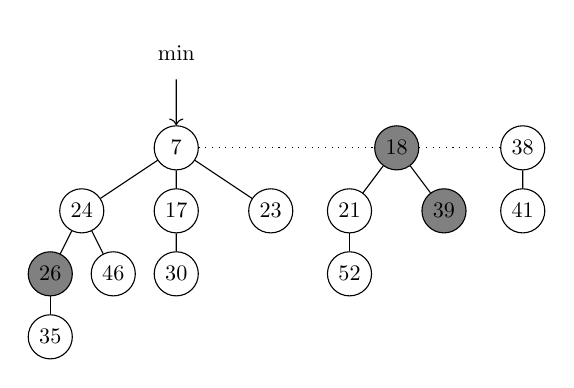
\begin{tikzpicture}
	[scale=0.80, transform shape, level distance=10mm,
	every node/.style={circle,draw,inner sep=2pt,minimum size=.7cm},
	level 1/.style={sibling distance=15mm},
	level 2/.style={sibling distance=10mm}]
	\node (7) at (0,0) {7}
	child {node {24}
		child {node [fill=gray] {26}
			child {node {35}}
		}
		child {node {46}	
	}}
	child {node {17}
		child {node {30}}}
	child {node {23}};
	\node (18) [fill=gray] at (3.5,0) {18}
	child {node {21}
	child {node {52}}}
	child {node [fill=gray]  {39}};
	\node (38) at (5.5,0) {38}
	child {node {41}};
	\draw [dotted] (7) -- (18) -- (38);
	\node (min) [draw=none] at (0,1.5) {min};
	\draw [->] (min) -- (7);
	\end{tikzpicture}
	\caption{}
	\label{fig:Fdeleteg}
\end{subfigure}
	\caption{Deleting the minimum element \cite{thomas2022}.}
	\label{fig:Fdelete}
\end{figure}
\FloatBarrier

\section{Relation to Fibonacci Numbers}
Fibonacci heaps derive their name from their connection to Fibonacci numbers, a relationship we explore in this section. The lemmas, corollaries, and proofs in this section are sourced and slightly adapted from the book \enquote{Introduction to Algorithms} of Cormen et al. \cite{thomas2022}. %page 526
%A tree of degree $r$ has at least $F_{r+2}$ nodes in it
\lemma\label{lem_19_1}{Let $x$ be any node in a Fibonacci heap, and suppose that $\texttt{getDegree}\ x = k$. Let $y_1,y_2,\dots,y_k$ denote the children of $x$ in the order in which they were linked to $x$, from the earliest to the latest. Then \texttt{getDegree} $y_1$ $\geq 0$ and \texttt{getDegree} $y_i$ $\geq i-2$ for $i = 2,3,\dots k$.}

\proof{Clearly, \texttt{getDegree} $y_1$ $\geq 0$.\\
For $i \geq 2$, we note that when $y_i$ was linked to $x$, all of $y_1,y_2,\dots y_{i-1}$ were children of $x$, and so we must have had \texttt{getDegree} $x$ $\geq i-1$. Because node $y_i$ is linked to $x$ (by \texttt{meld}) only if \texttt{getDegree} $x =$ \texttt{getDegree} $y_i$, we must have also had \texttt{getDegree} $y_i$  $\geq i-1$ at that time. Since then, node $y_i$ has lost at most one child, since it would have been cut from $x$ if it had lost two children. We conclude that  \texttt{getDegree} $y_i$ $\geq i-2$.
\qed}

The Fibonacci numbers are recursively defined for $k=0,1,2,\dots,$ as follows.
\[F_k = 
 \begin{cases}
0 & \text{if } k = 0\\
1 & \text{if } k = 1\\
F_{k-1} + F_{k-2} & \text{if } k \geq 2
\end{cases}   \]
Another way to calculate Fibonacci numbers is described in the following lemma.

\lemma{\label{lem_19_2}
For all integers $k\geq 0$,
\[ F_{k+2} = 1 + \sum_{i=0}^{k}F_i.\]}

\proof{Trivial by induction on $k$. \qed}

%\proof{The proof is by induction on $k$. When $k=0$,
%\begin{align*}
%	1+\sum_{i=0}^{0}F_i = 1 + F_0= F_1+F_0 = F_2.
%\end{align*}
%We now assume the inductive hypothesis that $F_{k+1} = \sum_{i=0}^{k-1}F_i$. In the step case we have
%\begin{align*}
%	1 + \sum_{i=0}^{k}F_i & = F_k + \left( 1+ \sum_{i=0}^{k-1}F_i  \right)\\
%	& = F_k + F_{k+1} = F_{k+2}	
%\end{align*}
%\qed}

\lemma{Let $x$ be any node in a Fibonacci heap, and let \texttt{getDegree} $x$ $= k$. Then \texttt{getSize} $x$ $\geq F_{k+2}$, where \texttt{getSize} $x$ is the number of nodes of the tree where $x$ is the root.}

\proof{
	Let $s_k$ denote the minimum possible size of any node of degree $k$ in any Fibonacci heap. Trivially, $s_0=1=F_2$ and $s_1=2=F_3$ and hence $s_k \geq F_{k+2}$ for $k=0$ and $k=1$. The number $s_k$ is at most \texttt{getSize} $x$ and, because adding children to a node cannot decrease the node's size, the value of $s_k$ increases monotonically with $k$. Consider some node $z$, in any Fibonacci heap, such that \texttt{getDegree} $z$ $= k$ and \texttt{getSize} $z$ $= s_k$. Because $s_k \leq$ \texttt{getSize} $x$, we compute a lower bound on \texttt{size}$(x)$ by computing a lower bound on $s_k$. As in Lemma \ref{lem_19_1}, let $y_1,y_2,\dots,y_k$ denote the children of $z$ in the order in which they were linked to $z$. To bound $s_k$, we add one to the count for $z$ itself and one for the first child $y_1$ (for which \texttt{getSize} $y_1$ $\geq 1)$. Additionally, we assume the induction hypothesis $s_i \geq F_{i+2}$ for $i = 0,1,...,k-1$, giving
\begin{align*}
	\texttt{getSize } x & \geq s_k \geq 2 + \sum_{i=2}^{k}{s_{(\texttt{getDegree } y_i)}} \overset{\text{Lem } \ref{lem_19_1}}{\geq} 2 + \sum_{i=2}^{k}{s_{i-2}} \\
	& \overset{\text{IH}}{\geq} 2 + \sum_{i=2}^{k}{F_i} = 1 + \sum_{i=0}^{k}{F_i} \overset{\text{Lem }\ref{lem_19_2}}{=} F_{k+2}.
\end{align*}
\qed}

\section{Comparison with Binomial Heaps}\label{fibheap_comparison}
Fibonacci heaps, like binomial heaps, consist of trees and support main operations such as inserting an element, merging heaps, finding, or deleting the minimum element in the heap. However, there are some differences between them.
Fibonacci heaps have less stringent invariants than binomial heaps. They allow multiple trees of the same degree in the tree list, and the list does not need to be ordered by it. 

\definition{\emph{Time complexity analysis} falls within computational complexity theory, serving to characterize how much computational resources an algorithm utilizes. The big-O notation denotes the maximum growth rate of a function and is used to express asymptotic behavior \cite{knuth1976big}.}

Moreover, as we will see in Chapter \ref{sec:amortized}, Fibonacci heaps offer better amortized costs than binomial heaps because they postpone expensive heap operations and execute them at a later point. In contrast to binomial heaps, Fibonacci heaps separate the tree with the minimum element from the tree list. Consequently, the function \texttt{findMin} in Fibonacci heaps has constant time complexity because it can directly access the tree with the minimum element as its root. 

From a theoretical perspective, Fibonacci heaps prove advantageous particularly when the occurrences of \texttt{deleteMin} and \texttt{delete} operations are comparatively low in relation to other operations \cite{thomas2022}. This scenario commonly arises across various applications. For instance, in certain greedy graph algorithms, such as Dijkstra's or Prim's algorithm.
Despite Fibonacci heaps outperforming binomial heaps in terms of asymptotic time bounds which is summarized in Table \ref{tab:amortized_cost}, they are primarily of theoretical interest due to their complex constant factors and programming intricacies \cite{thomas2022}. This is shown in experiments like network optimizations \cite{fredman1986pairing} or shortest path algorithms \cite{cherkassky1996shortest}, where a Fibonacci heap implementation did not perform as efficient as expected. This might be because constant factors of implementations in Fibonacci heaps are greater than those for binomial heaps. 


The representation of Fibonacci trees is similar to binomial trees, but each node in a Fibonacci heap also stores a Boolean indicating whether the node is marked or not.
In Section \ref{amortized_bin1}, we will prove that the length of a binomial heap can be bounded by the logarithm of the number of nodes in the heap. However, this result does not hold for Fibonacci heaps. For example, a Fibonacci heap could consist only of singletons, leading to a linear length in terms of the number of nodes in the heap.



\chapter{Amortized Analysis}\label{sec:amortized}
Time complexity analysis of algorithms and data structures can be conducted in various ways, including worst-case, average-case, and amortized runtime analysis.
Worst-case analysis determines the longest running time of an algorithm, providing an upper bound on the number of operations it takes to complete on any input. While worst-case analysis is essential for understanding an algorithm's behavior in extreme scenarios, it may not accurately represent typical real-world situations and can lead to overly pessimistic estimations.
Average-case runtime analysis calculates the expected number of operations an algorithm takes to complete over all possible inputs, considering a specific input distribution. However, this analysis requires accurate modeling of input distributions, which can be complex and may not reflect real-world scenarios \cite{tarjan1985amortized}.

Amortized runtime analysis, on the other hand, does not involve probabilistic considerations. It provides the average time taken per operation in a sequence of operations on a data structure or algorithm. This analysis is particularly useful for data structures supporting numerous operations, focusing on operation sequences rather than individual worst-case scenarios. Section \ref{fundamentals} provides an overview of the fundamentals of amortized analysis, drawing on descriptions and definitions from Cormen et al. \cite{thomas2022}. Here, we focus on the potential method of amortized analysis. Section \ref{amortized_bin1} conducts a concrete amortized cost analysis on binomial heaps, while Section \ref{sec:fibbound} performs a similar analysis on Fibonacci heaps.

\section{Fundamentals} \label{fundamentals}


Amortized analysis can be performed using different techniques, including aggregate analysis, the accounting method, and the potential method \cite{sadagopanAm}.
The aggregate analysis computes the average cost of a sequence of operations by distributing the total cost uniformly across all operations, providing a comprehensive evaluation of the algorithm's overall efficiency.
In the accounting method, each operation is assigned a credit, and the credits are used to compensate for the actual costs, ensuring that the total accumulated credits remain non-negative. This approach provides a formal mechanism for analyzing the average performance of a sequence of operations.
The potential method involves allocating a potential function to the data structure being analyzed, representing the stored \enquote{potential energy} that can be used to offset future operation costs. By comparing the potential before and after a sequence of operations, one can determine the amortized cost of operations, providing insights into the overall efficiency of the algorithm \cite{sadagopanAm}.
This thesis focuses exclusively on the potential function method for amortized cost analysis, and we provide a detailed explanation of this method in this section.

\definition{Let $D_i$ be the data structure that results after applying the $i$-th operation to data structure $D_{i-1}$ for $i = 1,2,\dots, n$ and $D_0$ be the initial data structure. A \textit{potential function} $\phi$ maps each data structure $D_i$ to a real number $\phi(D_i)$, which is the potential associated with data structure $D_i$.}

\definition{The \textit{amortized cost} $a_i$ of operation $i$ with respect to the potential function $\phi$ equals the actual cost $c_i$ of the $i$-th operation plus the increase in potential due to that operation:
	\[a_i  = c_i + \phi(D_i) - \phi(D_{i-1}).\]
}

Hence the total amortized cost of $n$ operations $A(D_n)$ is
\begin{align*}
A(D_n) = \sum_{i=1}^{n}a_i &= \sum_{i=1}^{n}(c_i + \phi(D_i) - \phi(D_{i-1})) \\
&= \sum_{i=1}^{n}c_i + \phi(D_n) - \phi(D_0) \\
&= T(D_n) + \phi(D_n) - \phi(D_0),
\end{align*}
where the total cost is denoted as $T(D_n)$.

\definition{The sum of amortized costs will be an \textit{amortized bound}, if it is an upper bound on the actual cost:
\[ A(D_n) = \sum_{i=1}^{n} a_i \geq \sum_{i=1}^{n} c_i = T(D_n).\]
}

We conclude that there is an amortized bound whenever $\phi(D_n) \geq \phi(D_0)$.
If the potential difference of an operation $i$ is positive, the amortized cost $a_i$ represents an overcharge and if it is negative it represents an undercharge to the operation and the potential of the data structure increases or decreases respectively.
As we can see from the definition, the amortized cost depends on the potential function. Changing the potential function results in different amortized costs and hence different upper bounds on actual costs.

Amortized cost analysis serves as a powerful tool in algorithmic evaluation, providing a nuanced perspective on computational efficiency over sequences of operations. By distributing costs and incorporating potential functions, this method enables comprehensive assessment of an algorithm's average performance. It can help to identify optimal strategies, to enhance our understanding of the long-term resource requirements, contributing to the refinement and optimization of algorithms in diverse scientific and computational domains \cite{tarjan1985amortized}.



\section{Binomial Heap Bounds}\label{amortized_bin1}
In this section, we establish an amortized bound for binomial heaps by conducting an amortized analysis using the potential function method. Our analysis builds upon the work presented in Okasaki's book \enquote{Purely functional data structures} \cite{okasaki1999}. First, we define the costs and potential function associated with our data structure.

\definition{The cost measure of \texttt{insTree}, \texttt{insert}, etc. is defined as the total number of (recursive) calls.}
\definition{\label{def:Bpot}Let the potential $\phi$ of a binomial heap $ts$ and a pair $(t,ts)$ of a binomial tree $t$ and heap $ts$ be defined as
\begin{align*}
	\phi(ts) &= l(ts)\\
	\phi((t,ts)) &= l(t:ts),
\end{align*} 
where $l(ts)$ and $l(t:ts)$ denotes the length of the heap $ts$ and $t:ts$ accordingly.}

To prove that the length of a binomial heap is bounded by the logarithm, we need some additional lemmas. First, we require the information that the length of the heap is bounded by the largest rank plus one which we denote in Lemma \ref{lem:lenLeRank}. Additionally, we need Corollary \ref{lem:sumRankProp} to convert a rank notation back to the number of nodes to complete the proof. By performing these steps, the proof of Lemma \ref{lem_log} presented in this thesis is a reduced, direct conversion of the proof done in Liquid Haskell.

\lemma{\label{lem:lenLeRank}Let $ts$ be a non-empty binomial heap. Then the length of $ts$ is bound by the greatest rank of the heap plus one:
	\[l(ts) \leq r_n + 1.\]
	Here $r_n$ denotes the rank of the last tree $t_n$ in the heap. Because the list is ordered by rank, $r_n$ is greatest rank of $ts$.}
\proof{The proof is by structural induction on $ts$. For $ts = [t_1]$ we have
\[l([t_1]) = 1 \leq r_1 + 1.\]
Because ranks are natural numbers, this case trivially holds. We assume the induction hypothesis $l(ts) \leq r_{n-1} + 1$ for $ts = [t_1,...,t_{n-1}]$. For $ts = [t_1,...,t_{n-1}, t_{n}]$ we have
\[l(ts) = n \leq r_{n-1} + 1 + 1 \leq r_{n} + 1.\]\\
The last relation holds because the list is ordered by rank and hence $r_{n-1} < r_{n}$.
\qed}

\lemma{\label{lem:pow2Lem}Let $t$ be a non-empty binomial tree with rank $r$. Then
	\[ 2^{r} = |t|,\]
where $|t|$ denotes the number of nodes of $t$.}
\proof{The proof is by induction on $r$.\\
For $r=0$: We know by definition that $t$ consists of only one node and hence
\[2^0 = 1 = |t|.\]
For $r=n+1$: Using our induction hypothesis and the information that a tree of rank $r+1$ consists of two binomial trees $t_1$ and $t_2$ of rank $r$ we conclude
\[2^{r+1} = 2^r + 2^r = |t_1| + |t_2| = |t|. \]
This is because we increase the rank only when linking two trees of the same rank.
\qed}

\corollary{\label{lem:sumRankProp}Let $ts = [t_1,...,t_n]$ be a non-empty binomial heap and $r_i$ denote the rank of a binomial tree $t_i$ in the heap. Then
\[|ts| = \sum_{i=1}^{n} 2^{r_i},\]
where $|ts|$ denotes the number of nodes of $ts$.}
\proof{This follows as a consequence of Lemma \ref{lem:pow2Lem}.
\qed}

\lemma{\label{lem_log}Let $ts$ be a binomial heap. Then the length of $ts$ is bound by the logarithm of the size of the heap plus one:
	\[l(ts) \leq \log_2(|ts|)+1.\]}
\begin{samepage}
\proof{The base case where $ts=[]$ trivially holds. Next, we consider a non-empty binomial heap and use the lemmas from before. Additionally, we apply rules of logarithm and sum. Note that $\log$ always refers to the logarithm of base two.
	\begin{align*}
	l(ts) &\leq r_n + 1 & \text{(by Lemma \ref{lem:lenLeRank})}\\
	&= \log 2^{r_n + 1} = \log 2^{r_n} + \log 2 \\
	&= \log 2^{r_n} + 1 \leq \log \left(\sum_{i=1}^{n} 2^{r_i}\right) +1  \\
	&= \log_2(|ts|)+1. & \text{(by Corollary \ref{lem:sumRankProp})}
	\end{align*}\qed}
\end{samepage}


While the \texttt{insert} function on binomial heaps runs in a worst-case time of $O(\log_2|ts|)$, it runs in constant amortized time \cite{okasaki1999}. To show that this holds we need to prove that \texttt{insTree} runs in $O(1)$ amortized time.

\lemma{\label{lem_insTree}Let $t$ be a binomial tree and $ts$ be a binomial heap. 
	\[ A(\texttt{insTree} \; t \; ts) \in O(1).\]}
\proof{It suffices to prove that $A(\texttt{insTree} \; t \; ts) \leq 1$. 

First, we consider the case where $\texttt{insTree} \; t \; ts = \texttt{insTree} \; (\texttt{link} \; t \; t') \; ts'$, which refers to the otherwise case in Line 8 of \Cref{fig:Binsert}. Then
\begin{align}
	A(\texttt{insTree} \; t \; ts) =\text{ }& T(\texttt{insTree} \; t \; ts) + \phi(\texttt{insTree} \; t \; ts) - \phi(ts) \label{eq4.1} \\
	=\text{ }& 1 + T(\texttt{insTree} \; (\texttt{link} \; t \; t') \; ts') + \phi(\texttt{insTree} \; t \; ts) - \phi(ts) \label{eq4.2}\\
	=\text{ }& 1 + A(\texttt{insTree} \; (\texttt{link} \; t \; t') \; ts') + \phi(ts') \nonumber\\
	 & - \phi(\texttt{insTree} \; (\texttt{link} \; t \; t') \; ts') + \phi(\texttt{insTree} \; t \; ts) - \phi(ts) \label{eq4.3}\\
	=\text{ }& 1 + A(\texttt{insTree} \; (\texttt{link} \; t \; t') \; ts') + l(ts') - l(ts) \label{eq4.4}\\
	=\text{ }& A(\texttt{insTree} \; (\texttt{link} \; t \; t') \; ts') \leq 1. \label{eq4.5}
\end{align}
In Equation \ref{eq4.1} we apply the definition of amortized cost. Equation \ref{eq4.2} steps with cost 1 into our considered case. We can rewrite the total costs by transforming the definition of amortized costs in Equation \ref{eq4.3}. Next, in Equation \ref{eq4.4}, we cancel both potentials of \texttt{insTree} and use the length of the heap according to the definition of the potential. In the last step we employ that by definition $l(ts) < l(ts')$. The result that the amortized cost in Equation \ref{eq4.5} is less than or equal to one follows by the case analysis.

Second, we consider the case $\texttt{insTree} \; t \; ts = t : ts$. This case, that can be seen in Line 7 of \Cref{fig:Binsert}, is non-recursive and hence it is easy to show that it has constant amortized time because the costs in this case are zero.
\begin{align*}
A(\texttt{insTree} \; t \; ts) &= T(\texttt{insTree} \; t \; ts) + \phi(\texttt{insTree} \; t \; ts) - \phi(ts)\\
&= \phi(t :ts) - \phi(ts) = l(t:ts) - l(ts) = 1.
\end{align*}
\qed}
\lemma{Let $x$ be an element and $ts$ be a binomial heap. 
	\[A(\texttt{insert} \; x \; ts) \in O(1).\]}
\proof{By definition of the function we have $\texttt{insert} \; x \; ts = \texttt{insTree}$ (Node 0 $x$ []) $ts$ and since the amortized cost of \texttt{insTree} is in constant time by Lemma \ref{lem_insTree}, the same holds for the \texttt{insert} function.
\qed}

\lemma{Let $ts_1$ and $ts_2$ be binomial heaps. 
	\[A(\texttt{merge} \; ts_1 \; ts_2) \in O(\log_2(|ts_1|+|ts_2|)).\]}
\proof{\label{lem_merge}In order to prove the lemma, we prove the stronger claim 
\[ A(\texttt{merge} \; ts_1 \; ts_2) \leq l(ts_1) + l(ts_2). \]
First, consider the claim and the case $\texttt{merge} \; ts_1 \; ts_2 = \texttt{insTree} \; (\texttt{link} \;t\;t')\;(\texttt{merge} \; ts_1' \; ts_2')$ which corresponds to the otherwise case in Line 6 of \Cref{fig:Bmerge}. Whenever we have two or more input data structures, $\phi(D_0)$ equals the sum of all input potentials which in this case is $\phi(ts_1) + \phi(ts_2)$.
Then
\begin{align}
	A(\texttt{merge} \; ts_1 \; ts_2) =\text{ }& T(\texttt{merge} \; ts_1 \; ts_2) + \phi(\texttt{merge} \; ts_1 \; ts_2) - \phi(ts_1) - \phi(ts_2) \label{eq4.6}\\
	=\text{ }& 1 + T(\texttt{insTree} \; (\texttt{link} \;t\;t')\;(\texttt{merge} \; ts_1' \; ts_2')) + T(\texttt{merge} \; ts_1' \; ts_2') \nonumber\\
	& + \phi(\texttt{insTree} \; (\texttt{link} \;t\;t')\;(\texttt{merge} \; ts_1' \; ts_2')) - \phi(ts_1) - \phi(ts_2)  \label{eq4.7}\\
	=\text{ }& 1 + A(\texttt{insTree} \; (\texttt{link} \;t\;t')\;(\texttt{merge} \; ts_1' \; ts_2')) \nonumber\\
	& + \phi(\texttt{merge} \; ts_1' \; ts_2') - \phi(\texttt{insTree} \; (\texttt{link} \;t\;t')\;(\texttt{merge} \; ts_1' \; ts_2')) \nonumber\\
	& + A(\texttt{merge} \; ts_1' \; ts_2') + \phi(ts1')+\phi(ts2') - \phi(\texttt{merge} \; ts_1' \; ts_2') \nonumber\\
	& + \phi(\texttt{insTree} \; (\texttt{link} \;t\;t')\;(\texttt{merge} \; ts_1' \; ts_2')) - \phi(ts_1) - \phi(ts_2)  \label{eq4.8}\\
	=\text{ }& 1 + A(\texttt{insTree} \; (\texttt{link} \;t\;t')\;(\texttt{merge} \; ts_1' \; ts_2')) \nonumber\\
	&+ A(\texttt{merge} \; ts_1' \; ts_2') + \phi(ts1')+\phi(ts2') - \phi(ts_1) - \phi(ts_2)  \label{eq4.9}\\
	=\text{ }& 1 + A(\texttt{insTree} \; (\texttt{link} \;t\;t')\;(\texttt{merge} \; ts_1' \; ts_2')) \nonumber\\
	&+ A(\texttt{merge} \; ts_1' \; ts_2') - 2 \label{eq4.10}\\
	\leq \text{ }& 1 + 1 + l(ts_1') + l(ts_2') - 2 \leq l(ts_1) + l(ts_2).
\end{align}
Equation \ref{eq4.6} applies the definition of amortized cost. Since we consider exactly this case, our costs consist of the cost of the insertion of a tree as well as the costs of merging two smaller heaps. This can be seen in Equation \ref{eq4.7}, where we additionally add the number one for stepping into this case. Next, we rewrite the costs, which results in Equation \ref{eq4.8}. In Equation \ref{eq4.9} we canceled $\phi(\texttt{merge} \; ts_1' \; ts_2')$ and $\phi(\texttt{insTree} \; (\texttt{link} \;t\;t')\;(\texttt{merge} \; ts_1' \; ts_2'))$ because adding and then subtracting them is redundant. Since the potential corresponds to the length of the heap and the length of $ts_1'$ and $ts_2'$ is each one less than the length of the heap $ts_1$ and $ts_2$ respectively, we know that adding the potentials results in negative two in Equation \ref{eq4.10}. In the last step we used the claim and the result that \texttt{insTree} has constant amortized time of Lemma \ref{lem_insTree}. 

Second, consider the case $\texttt{merge} \; ts_1 \; ts_2 = t_1 : (\texttt{merge} \; ts_1' \; ts_2)$ of Line 4 of \Cref{fig:Bmerge}. Then
\begin{align*}
	A(\texttt{merge} \; ts_1 \; ts_2) =\text{ }& T(\texttt{merge} \; ts_1 \; ts_2) + \phi(\texttt{merge} \; ts_1 \; ts_2) - \phi(ts_1) - \phi(ts_2)\\
	=\text{ }& 1 + T(\texttt{merge} \; ts_1' \; ts_2)\;+ \phi(t_1:(\texttt{merge} \; ts_1' \; ts_2)) - \phi(ts_1)-\phi(ts_2) \\
	=\text{ }& 1 + A(\texttt{merge} \; ts_1' \; ts_2)\;+\phi(ts_1')+\phi(ts_2)-\phi(\texttt{merge} \; ts_1' \; ts_2)\\ &+\phi(t_1:(\texttt{merge} \; ts_1' \; ts_2)) - \phi(ts_1)-\phi(ts_2)\\
	=\text{ }& 1 + A(\texttt{merge} \; ts_1' \; ts_2) \\
	\leq\text{ }& 1 + l(ts_1') + l(ts_2) = l(ts_1) + l(ts_2).
\end{align*}

Third, consider the case $\texttt{merge} \; ts_1 \; ts_2 = t_2 : (\texttt{merge} \; ts_1 \; ts_2')$ of Line 5 of \Cref{fig:Bmerge}, which can be proven analogously to the former case. This completes the proof of the stronger claim and because we know that the length of a heap is logarithmic in the size of the heap by Lemma \ref{lem_log}, we conclude
\begin{align*}
	A(\texttt{merge}\;ts_1\;ts_2) &\leq l(ts_1)+l(ts_2) \\
	& \leq \log_2(|ts_1|) + \log_2(|ts_2|) + 2\\
	& \in O(\log_2(|ts_1|+|ts_2|)).
\end{align*}
\qed
}

\lemma{\label{lem_remTree}Let $ts$ be a binomial heap.
	\[A(\texttt{removeMinTree} \; ts) \in O(\log_2(|ts|)).\]}
\proof{As before, we first prove the stronger claim that $A(\texttt{removeMinTree} \; ts) \leq l(ts)$ and then the result follows by application of Lemma \ref{lem_log}.

First, consider $\texttt{removeMinTree} \; (t:ts) = (t',t:ts')$ which is the else case of Line 4 of \Cref{fig:Bdelete} where $\texttt{removeMinTree} \; ts = (t',ts')$. Here we do the same as in the proofs before. We begin by applying the definition of amortized costs, then we rewrite the total costs and finally cancel the potentials by using the invariant that $l(ts) = l(t':ts')$.
\begin{align*}
	A(\texttt{removeMinTree} \; (t:ts)) =\text{ }& T(\texttt{removeMinTree} \; (t:ts)) + \phi(\texttt{removeMinTree} \; (t:ts)) \\
	&- \phi(t:ts) \\
	=\text{ }& 1 + T(\texttt{removeMinTree} \; ts) + \phi((t',t:ts'))-\phi(t:ts) \\
	=\text{ }& 1 + A(\texttt{removeMinTree} \; ts) + \phi(ts) - \phi((t',ts')) \\
	&+ \phi((t',t:ts'))-\phi(t:ts) \\
	=\text{ }& 1 + A(\texttt{removeMinTree} \; ts) \leq 1 + l(ts) = l(t:ts).
\end{align*}
Second, consider $\texttt{removeMinTree} \; (t:ts) = (t,ts)$, which is the then case of Line 4 of \Cref{fig:Bdelete}. We perform the same steps as in the first case.
\begin{align*}
A(\texttt{removeMinTree} \; (t:ts)) &= T(\texttt{removeMinTree} \; (t:ts)) + \phi(\texttt{removeMinTree} \; (t:ts)) \\
&- \phi(t:ts) \\
&= 1 + T(\texttt{removeMinTree} \; ts) + \phi((t,ts))-\phi(t:ts) \\
&= 1 + A(\texttt{removeMinTree} \; ts) + \phi(ts) - \phi((t',ts')) \\
&+ \phi((t,ts))-\phi(t:ts) \\
&= 1 + A(\texttt{removeMinTree} \; ts) \leq 1 + l(ts) = l(t:ts).
\end{align*}
Hence we conclude that $A(\texttt{removeMinTree} \; ts) \in O(\log_2(|ts|))$ holds.
\qed
}

\corollary{Let $ts$ be a binomial heap. \[A(\texttt{findMin} \; ts) \in O(\log_2(|ts|)).\]}
\proof{The proof follows directly from the definition of \texttt{findMin} and Lemma \ref{lem_remTree}. \qed }

\lemma{Let $ts$ be a binomial heap. 
	\[A(\texttt{deleteMin} \; ts) \in O(\log_2(|ts|)).\]}
\proof{The claim follows essentially as a consequence of Lemma \ref{lem_merge} and Lemma \ref{lem_remTree}. 
	First, we again apply the definition of amortized cost in Equation \ref{eq4.12}. Next, we split up the actual costs in Equation \ref{eq4.13} to be the costs of \texttt{removeMinTree} and \texttt{merge} because of the functions definition that can be seen in \Cref{fig:Bdelete}. Equation \ref{eq4.14} then rewrites the cost by transforming the definition of amortized cost. We employ the definition $\texttt{deleteMin}\;ts = \texttt{merge}\;(\texttt{reverse}\;ts_1)\;ts_2$ and cancel equal terms in Equation \ref{eq4.15}. In the last steps we apply the definition of the potential function $\phi$. Because $l(ts_2) \leq l((\text{Node }r \; x \;ts_1):ts_2)$ and a reverse list has the same length as the list itself, we can simplify the equation and apply Lemma \ref{lem_log} and the amortized costs from Lemma \ref{lem_merge} and Lemma \ref{lem_remTree}.
\begin{align}
A(\texttt{deleteMin} \; ts) =\text{ }& T(\texttt{deleteMin} \; ts) + \phi(\texttt{deleteMin} \; ts) - \phi(ts) \label{eq4.12}\\
=\text{ }& T(\texttt{removeMinTree} \; ts) + T(\texttt{merge}\;(\texttt{reverse} \; ts_1)\; ts_2) \nonumber\\
&+ \phi(\texttt{deleteMin} \; ts) - \phi(ts) \label{eq4.13}\\
=\text{ }& A(\texttt{removeMinTree} \; ts) + \phi(ts) - \phi((\text{Node } r \;x \;ts_1), ts_2) \nonumber\\
&+ A(\texttt{merge}\;(\texttt{reverse} \; ts_1)\; ts_2) + \phi(\texttt{reverse} \; ts_1) + \phi(ts_2) \nonumber\\
&- \phi(\texttt{merge}\;(\texttt{reverse} \; ts_1)\; ts_2) + \phi(\texttt{deleteMin} \; ts) - \phi(ts) \label{eq4.14}\\
=\text{ }& A(\texttt{removeMinTree} \; ts) -  \phi((\text{Node } r \; x \;ts_1), ts_2)\nonumber\\
&+ A(\texttt{merge}\;(\texttt{reverse} \; ts_1)\; ts_2) + \phi(\texttt{reverse} \; ts_1) + \phi(ts_2)\label{eq4.15}\\
\leq \text{ }& A(\texttt{removeMinTree} \; ts) + A(\texttt{merge}(\texttt{reverse} \; ts_1)\; ts_2) \nonumber\\
&+ l(\texttt{reverse} \; ts_1) \nonumber\\
\leq\text{ }& A(\texttt{removeMinTree} \; ts) + A(\texttt{merge}(\texttt{reverse} \; ts_1)\; ts_2) + c_3 \cdot \log_2(|ts_1|)\nonumber\\
\leq \text{ }& c_1 \cdot \log_2(|ts|) + c_2 \cdot \log_2(|ts_1|+|ts_2|)+ c_3 \cdot \log_2(|ts_1|) \in O(\log_2(|ts|)).\nonumber
\end{align}
\qed}

\section{Fibonacci Heap Bounds}\label{sec:fibbound}
Similarly to the previous section, we start by defining the cost measure and potential function of Fibonacci heaps to give amortized bounds for them. Our definitions, examples and lemmas are based on Cormen et al. \cite{thomas2022}.

\definition{The cost measure of \texttt{insert}, \texttt{merge}, etc. is defined as the total number of (recursive) calls.}
\definition{Let the potential $\phi$ of a Fibonacci heap $h$ be defined as
\begin{align*}
	\phi(h) = l(h) + 2 \cdot m(ts),	
\end{align*}
where $l(ts)$ denotes the length of the heap, which is the length of the trees plus one for the minimum tree,  and $m(ts)$ denotes the number of marked nodes in $ts$.
}
\example{To create an empty Fibonacci heap $h$ we just return $E$. Because the length of this Fibonacci heap is zero and we cannot have any marked nodes, since there are no nodes in the heap, the potential of an empty Fibonacci heap $h$ is $\phi(h) = 0$.}
\example{Consider the Fibonacci heap of Figure \ref{fig:exfib}. Here we have five trees in our root list including the minimum tree. Moreover, three nodes are marked. Hence the potential of this Fibonacci heap is $5+2 \cdot 3 = 11$.}

\lemma{\label{lem_bound}Let $h$ be a Fibonacci heap. Then 
	\[ D(h) \leq \lfloor\log_2 |h| \rfloor,\] 
where $D(h)$ denotes the the maximum degree of $h$ and $|h|$ denotes the number of nodes of $h$ und $\lfloor \cdot \rfloor$ denotes the floor function \cite{thomas2022}.}
\proof{
For $h = []$ the claim $D(h) \leq \lfloor\log_2 |h| \rfloor$ trivially holds.
The only case where the degree of a heap and hence also the maximum degree $D(h)$ increase, is if the \texttt{link} function is called. This function is only called when melding the heap. After melding, all trees have a unique degree and the Fibonacci heap can be seen as a binomial heap. Hence the proof is analogous to the proof of Lemma \ref{lem_log} where the greatest rank $r_n$ corresponds to the maximum degree $D(h)$.
\qed}

Further, we show amortized bounds for Fibonacci heap functions. While the functions \texttt{insert}, \texttt{merge} and \texttt{findMin} have constant amortized time, the \texttt{deleteMin} function has a logarithmic bound.

\lemma{\label{lem_Fmerge}Let $h_1$ and $h_2$ be a Fibonacci heaps. 
	\[A(\texttt{merge}\;h_1\;h_2) \in O(1).\]}
\proof{Consider the case $\texttt{merge}\;h_1\;h_2 = \text{FH }minTr_1\;(minTr_2:ts_2$\lstinline|++|$ts_1)$ of Line 6 in \Cref{fig:Fcode1}. Then
\begin{align}
	A(\texttt{merge}\;h_1\;h_2) =\text{ }& T(\texttt{merge}\;h_1\;h_2) + \phi(\texttt{merge}\;h_1\;h_2) - \phi(h_1) - \phi(h_2) \label{eq4.16}\\
	=\text{ }& 1 + \phi(\texttt{merge}\;h_1\;h_2) - \phi(h_1) - \phi(h_2) \label{eq4.17}\\
	=\text{ }& 1 + l(\texttt{merge}\;h_1\;h_2) + 2 \cdot m(\texttt{merge}\;h_1\;h_2))) \nonumber\\
	&- (l(h_1) + 2 \cdot m(h_1)) - (l(h_2) + 2 \cdot m(h_2)) \label{eq4.18}\\
	=\text{ }& 1 + 2 \cdot m(\texttt{merge}\;h_1\;h_2))) - 2 \cdot m(h_1) - 2 \cdot m(h_2) \label{eq4.19}\\
	=\text{ }& 1. \label{eq4.20}
\end{align}
First, we apply the definition of amortized cost in Equation \ref{eq4.16}. Since the function \texttt{merge} is non-recursive we simply have a total cost of one in Equation \ref{eq4.17} to step into our case. In Equation \ref{eq4.18} we employ the definition of our potential function, which is the length added by twice the number of marked nodes. Moreover, in Equation \ref{eq4.19} we employ $l(\texttt{merge}\;h_1\;h_2) = l(h_1) + l(h_2)$ and therefore we can cancel it. Last, we know that $m(\texttt{merge}\;h_1\;h_2) = m(h_1) + m(h_2)$ because we do not change any marked nodes in this function, which results in an amortized cost of constant one in Equation \ref{eq4.20}.

Second, the other case where $\texttt{merge}\;h_1\;h_2 = \text{FH }minTr_2\;(minTr_1:ts_1$\lstinline|++|$ts_2)$ is analogous.
\qed
}
\lemma{Let $h_1$ and $h_2$ be Fibonacci heaps. 
	\[A(\texttt{insert}\;h_1\;h_2) \in O(1).\]}
\proof{This is a direct result from Lemma \ref{lem_Fmerge}. Since the function \texttt{singleton} is just a single call with cost one and we know that \texttt{merge} has constant amortized time we get that \texttt{insert} has constant amortized time. \qed}

\lemma{Let $h$ be a Fibonacci heap.
\[A(\texttt{findMin}\;h) \in O(1).\]}
\proof{Finding the minimum node of a Fibonacci heap is in $O(1)$ actual time. This is because we store minTree separately and can directly access the root node of it. Because there is no change in potential of our heap, it follows that the actual cost equals the amortized cost \cite{thomas2022}.
\qed}

In the function \texttt{deleteMin} we delete the minimum element and add its children to the root list. Then we link trees with the same degree. Since the data structure is implemented with pointers in the literature they have direct access to parents, siblings, etc.. Moreover, \texttt{consolidate} uses an array that stores the trees by degree and links them whenever there is already a tree with the same degree. However, with our functional implementation we have to iterate through the list again and again until we reach that result. Therefore, we do not count those extra costs but rather refer to the actual costs in the literature \cite{thomas2022}.

\lemma{Let $h$ be a Fibonacci heap. 
	\[A(\texttt{deleteMin}^*\;h) \in O(log_2(|h|)).\]}
\proof{
 The function $\texttt{deleteMin}^*$ refers to an imperative implementation of our \texttt{deleteMin} that uses pointers and arrays and has a total cost of $T(\texttt{deleteMin}^*\;h) = l(h)+D(h)$ according to the literature. Moreover, $l(\texttt{deleteMin}^*\;h) = D(h) + 1$ and $m(\texttt{deleteMin}^*\;h) = 2 \cdot m(h)$ because at most $D(h) + 1$ roots remain and no nodes become marked during the operation \cite{thomas2022}. In the last step of the proof we apply Lemma \ref{lem_bound}.
\begin{align*}
	A(\texttt{deleteMin}^*\;h) =\text{ }& T(\texttt{deleteMin}^*\;h) + \phi(\texttt{deleteMin}^*\;h) - \phi(h)\\
	=\text{ }& l(h) + D(h) + \phi(\texttt{deleteMin}^*\;h) - \phi(h)\\
	=\text{ }& l(h) + D(h) +(l(\texttt{deleteMin}^*\;h)+2 \cdot m(\texttt{deleteMin}^*\;h)) \\
	&- (l(h) + 2 \cdot m(h))\\
	=\text{ }& l(h) + D(h) + D(h) + 1 + 2 \cdot m(h) - (l(h) + 2 \cdot m(h))\\
	=\text{ }& D(h) + D(h) + 1 \in O(\log_2(|h|)).
\end{align*}
\qed}

Finally, we summarize our results of Section \ref{amortized_bin1} and Section \ref{sec:fibbound} in Table \ref{tab:amortized_cost}.
\begin{table}[h]
	\centering
	\caption{Amortized analysis of binomial heap and Fibonacci heap.}
	\begin{tabular}{lcc}
		Heap Operation & Binomial heap $ts$ & Fibonacci heap $h$ \\
		\hline
		\texttt{makeHeap} & $O(1)$ & $O(1)$ \\
		\texttt{insert} & $O(1)$  & $O(1)$ \\
		\texttt{merge} & $O(1)$ & $O(1)$ \\
		\texttt{findMin} & $O(\log_2(|ts|))$  & $O(1)$ \\
		\texttt{deleteMin} & $O(\log_2(|ts|))$ & $O(\log_2(|h|))$ \\
		\hline
	\end{tabular}
	 \label{tab:amortized_cost}
	\end{table}

%\corollary{The maximum rank of any node in an $n$-node Fibonacci heap is $O(\log n)$.}

\chapter{Liquid Haskell}
Liquid Haskell represents an advanced type checker and refinement type system extension for the Haskell programming language. Developed as an open-source project, Liquid Haskell aims to provide developers with a more precise and formal approach to specifying and verifying the correctness of Haskell programs. By introducing refinement types, Liquid Haskell enables programmers to articulate detailed assertions about the properties that data should uphold, surpassing the capabilities of the traditional Haskell type system \cite{vazou2014liquidhaskell}.

The pivotal feature of Liquid Haskell lies in its capability to statically verify these refined types during the compilation process. This static verification aids in detecting potential errors and bugs early in the development cycle, providing developers with a powerful tool to ensure the correctness and reliability of their Haskell code. Liquid Haskell extends the advantages of formal verification to Haskell programs, enabling developers to express and verify involved properties of their code without the need for runtime checks \cite{pena2017}.

Liquid Haskell has found applications across various domains, including critical systems where correctness is paramount. By enabling developers to provide more detailed specifications for their functions and data, Liquid Haskell contributes to writing safer, more resilient code. While the adoption of refinement types and formal verification may entail a learning curve, the heightened assurance in the correctness of Haskell programs can be invaluable, particularly in contexts where software reliability is of utmost importance \cite{vazou2014liquidhaskell}.

In this chapter, we explain the setup and workflow of Liquid Haskell in Section \ref{sec:setup}, provide an introduction to refinement types in Section \ref{refinement}, followed by an introduction to proving extrinsic theorems in Section \ref{lh_proof}. Subsequently, we discuss the formalization of the refinements of binomial heap and Fibonacci heap functions in Section \ref{formalization_ref}. Finally, we introduce the \texttt{Tick} library to perform an amortized cost analysis in Section \ref{lh_eff}.

\section{Setup and Workflow}\label{sec:setup}
Before examining refinements and specifications, we explain the workflow of Liquid Haskell and our setup.
To utilize Liquid Haskell, we require an SMT solver installed on our system, such as the Z3 theorem prover from Microsoft Research\footnote{https://github.com/Z3Prover/z3}. Liquid Haskell itself is installed and enabled by adding it as a dependency in the project's \lstinline|cabal| file. Since we are using the Glasgow Haskell Compiler (GHC) version 9.0.1 for our project, we need to add both \texttt{liquidhaskell} and \texttt{liquid-base} to the build dependencies. This prompts \lstinline|cabal| to automatically:
\begin{enumerate}
	\item install Liquid Haskell,
	\item instruct GHC to use Liquid Haskell during compilation,
	\item display liquid type errors during compilation,
	\item integrate Liquid Haskell with \lstinline|ghcid| for Visual Studio Code.
\end{enumerate}
With this setup, Liquid Haskell can be executed either from the command-line\footnote{https://hackage.haskell.org/package/liquidhaskell} or within a web browser\footnote{http://goto.ucsd.edu/liquid/haskell/demo}. The workflow is illustrated in Figure \ref{fig:workflow}. According to Vazou et al. \cite{vazou2014liquidhaskell}, Liquid Haskell requires three inputs:
\begin{enumerate}
	\item A single Haskell source file containing both code and refinement type specifications,%, including refined datatype definitions, measures, predicate and type aliases, and function signatures
	\item A set of directories containing imported modules (including the Prelude) that may themselves contain specifications for exported types and functions,
	\item A set of predicate fragments called qualifiers, which are utilized to infer refinement types. This set is usually empty, as the default set of qualifiers extracted from the type specifications is typically sufficient for inference.
\end{enumerate}  

\begin{figure}[h]
	\centering
	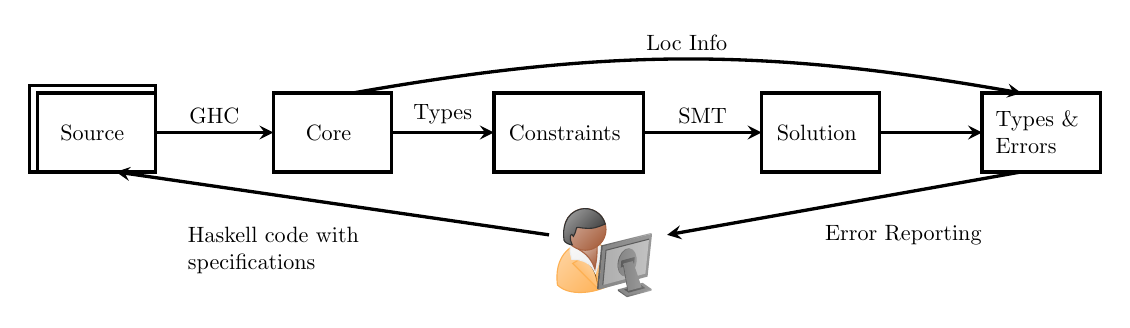
\begin{tikzpicture}
		\draw[black, very thick] (0,0) rectangle (1.5,1);
		\draw[black, very thick] (-0.1,0) rectangle (1.5,1.1);
		\draw[black, very thick] (3,0) rectangle (4.5,1);
		\draw[black, very thick] (5.8,0) rectangle (7.7,1);
		\draw[black, very thick] (9.2,0) rectangle (10.7,1);
		\draw[black, very thick] (12,0) rectangle (13.5,1);
		
		\node[align=left, scale=0.8] (1) at (0.7,0.5) {Source};
		\node[align=left, scale=0.8] (2) at (3.7,0.5) {Core};
		\node[align=left, scale=0.8] (3) at (6.7,0.5) {Constraints};
		\node[align=left, scale=0.8] (4) at (9.9,0.5) {Solution};
		\node[align=left, scale=0.8] (5) at (12.7,0.5) {Types \& \\ Errors};

		\draw[-stealth, very thick] (1.5,0.5) -- (3,0.5) node [scale= 0.8, pos=0.5, above] {GHC};
		\draw[-stealth, very thick] (4.5,0.5) -- (5.8,0.5) node [scale= 0.8, pos=0.5, above] {Types};
		\draw[-stealth, very thick] (7.7,0.5) -- (9.2,0.5) node [scale= 0.8, pos=0.5, above] {SMT};
		\draw[-stealth, very thick] (10.7,0.5) -- (12,0.5);
		\draw[-stealth, very thick] (4,1) to [bend left=10] node [scale= 0.8, pos=0.5, above, sloped] {Loc Info} (12.5,1);
		
		\node[alice, monitor, minimum size=0.8cm] (6) at (7,-1) {};
		\draw[-stealth, very thick] (12.5,0) -- (8,-0.8);
		\draw[stealth-, very thick] (1,0) -- (6.5,-0.8);
		
		\node[scale= 0.8] (7) at (11,-0.8) {Error Reporting};
		\node[align=left, scale= 0.8] (8) at (3,-1) {Haskell code with \\ specifications};

	\end{tikzpicture}
	\caption{Liquid Haskell workflow \cite{vazou2014liquidhaskell}.}
	\label{fig:workflow}
\end{figure}

The workflow of Liquid Haskell involves several procedural steps aimed at verifying the correctness of Haskell programs. Initially, GHC is utilized to transform the source code into its Core representation, as depicted in Figure \ref{fig:workflow}. Additionally, a mapping from Core expressions to corresponding locations in the Haskell source is established to facilitate simpler error reporting at the source level. Subsequently, the abstract interpretation framework of Liquid Typing \cite{rondon2008liquid}, adapted for soundness under lazy evaluation, is employed to derive logical constraints from the Core Intermediate Language (IL). These constraints are then resolved using a fixpoint algorithm in conjunction with an SMT solver, resulting in the deduction of a valid refinement typing for the program \cite{vazou2016liquid}.

In terms of output, Liquid Haskell categorizes the program as SAFE if the set of constraints is satisfiable, signifying successful verification. Conversely, if the constraints prove unsatisfiable, it outputs UNSAFE. Invalid constraints are instrumental in identifying and reporting refinement type errors, pinpointing the source positions that contributed to their creation. The process leverages location information to establish a mapping between the invalid constraints and the corresponding source positions. In either outcome, Liquid Haskell generates a source map containing inferred types for each program expression, a crucial component for debugging code and specifications \cite{vazou2014liquidhaskell}.

\FloatBarrier

\section{Refinement Types}\label{refinement}
Refinement types, also called liquid types or refinements, enable programmers to specify complex invariants by extending type systems with logical predicates \cite{vazou2014liquidhaskell}. We intuitively employed refinements in \Cref{fig:Bitree} and \Cref{fig:Biheap} to refine a binomial heap, and in \Cref{fig:fibtree} and \Cref{fig:fibheap} for Fibonacci heaps. These refinements allow us to specify properties like the order of ranks. Previously, when refining Fibonacci trees, we assumed refinement types like \textbf{Pos} without formally defining them. In this section, we delve into the basics of refinements.
Liquid types complement the standard Haskell type. Typically, they are written as comments in the form of \texttt{\{-$@$ annotation $@$-\}}. While GHC ignores these comments, Liquid Haskell processes them. For simplicity, we omitted this notation in previous examples, but we use it from this point to better distinguish between the Haskell type and the refinement type.

To illustrate the concept, we start by defining the previously mentioned type \textbf{Pos} shown in Line 1 of \Cref{fig:reftypes}. The $\textbf{Pos}$ type encompasses all positive integers, as the logical predicate specifies that values \texttt{v} of type $\textbf{Int}$ must be greater than zero. We provide additional examples of refinement types in \Cref{fig:reftypes}, defining non-empty tree lists and non-empty heaps. In these cases, the length of the list or heap must be greater than zero. This showcases how setting a refinement type in such cases is straightforward.


\begin{figure}[h]
\begin{lstlisting}[mathescape=true, language=haskell, caption={Refinement types.},captionpos=b, label=fig:reftypes]
$\LHl$ type $\textbf{Pos}$ = {v: Int | 0 < v} $\LHr$
$\LHl$ type $\textbf{NEBiTreeL a}$ = {xs:$\textbf{[BiTree a]}$ | $\texttt{len}$ xs > 0} $\LHr$
$\LHl$ type $\textbf{NEFibTreeL a}$ = {xs:$\textbf{[FibTree a]}$ | $\texttt{len}$ xs > 0} $\LHr$
$\LHl$ type $\textbf{NEBiHeap a}$	= {ts:$\textbf{BiHeap a}$ | $\texttt{len}$ ts > 0} $\LHr$
\end{lstlisting}
\end{figure}
Refinement types serve to enrich the types of functions, offering to specify more precise constraints. Take, for instance, the \texttt{insTree} function of binomial heaps described in \Cref{fig:Binsert}. Here, we can specify that the input is not just a list of binomial trees but actually a heap. Furthermore, we can refine the output of the function to be of the refinement type \textbf{NEBiHeap a} because we guarantee that at least one tree is inserted. We can even express that the length of the output is exactly one tree larger than the input heap. In the following code snippet (\Cref{fig:refinsTree}), we provide both the Haskell type annotation as well as the Liquid Haskell type.

\begin{figure}[h]
\begin{lstlisting}[mathescape=true, language=haskell, caption={Refinement \texttt{insTree}.},captionpos=b, label=fig:refinsTree]
$\LHl$ $\texttt{insTree}$ :: $\textbf{BiTree a}$ -> {$ts:\textbf{BiHeap a}$} 
	-> {$zs:\textbf{NEBiHeap a}$ | length $zs \leq$ length $ts + 1$} $\LHr$
$\texttt{insTree}$ :: Ord a => $\textbf{BiTree a}$ -> $\textbf{[BiTree a]}$ -> $\textbf{[BiTree a]}$
\end{lstlisting}
\end{figure}

In situations, where we forget to define the refined type to the function, Liquid Haskell raises a totality error due to non-exhaustive pattern matches. This scenario might arise, for example, in the \texttt{removeMinTree} function because the case for an empty list as input is not defined. Thus, calling \texttt{removeMinTree }[] would trigger a pattern error if we neglect to refine the input to be of type \textbf{NEBiHeap a}. Therefore, Liquid Haskell ensures that such errors are caught at compile-time rather than manifesting at runtime.

Liquid Haskell also enables functions to refine types, as demonstrated in \Cref{fig:fibtree}, where we utilized the function \texttt{equalDepth} to refine the type of the subtrees of a Fibonacci tree. If we intend to incorporate such a function in the type annotation, we must lift it into the refinement logic, meaning the function must be integrated into the logical framework of the refinement type system using either \textbf{measure} or \textbf{reflect}.
Measure replicates a Haskell function into the refinement logic, assigns an inferred refinement type to the constructor of the function's first argument, and generates an inferred global invariant associated with the refinement \cite{vazou2014liquidhaskell}.
Reflect generates an uninterpreted function with identical name in the refinement logic. It duplicates the implementation to a refinement type alias and appends a refinement to the type of the uninterpreted function that specifies the type alias as a post-condition \cite{vazou2017refinement}.
In both cases, all parts of the function definition must already be available to the refinement logic. While \textbf{measure} restricts lifting functions to those with a single argument and those that may structurally recurse on the single argument, \textbf{reflect} is less restrictive, permitting recursive functions and multiple arguments \cite{vazou2014liquidhaskell}. %\footnote{https://ucsd-progsys.github.io/liquidhaskell/specifications/}

For example, to use the Haskell Prelude function \texttt{length} for the type \textbf{\lstinline{NEBiHeap a}} or \textbf{\lstinline{NEHeap a}}, we must lift it. Alternatively, we can employ the function \texttt{len}, which is already defined as a measure in the Liquid Haskell Prelude.

In \Cref{fig:measure}, we demonstrate the process of lifting the function \texttt{emptyFibHeap}. Once we add \texttt{emptyFibHeap} as a measure, we can seamlessly utilize it in the annotation to refine the types \textbf{\lstinline{NEFibHeap}} and \textbf{\lstinline{EFibHeap}} without encountering any issues.
\begin{figure}[h]
\begin{lstlisting}[mathescape=true, language=haskell, caption={Measure \texttt{emptyFibHeap}.},captionpos=b, label=fig:measure]
$\LHl$ $\textbf{measure}$ $\texttt{emptyFibHeap}$ $\LHr$
$\texttt{emptyFibHeap}$ :: $\textbf{FibHeap a}$ -> Bool
$\texttt{emptyFibHeap}$ E = True
$\texttt{emptyFibHeap}$ _ = False

$\LHl$ type $\textbf{NEFibHeap}$ = {v : $\textbf{FibHeap a}$ | not $\texttt{emptyFibHeap}$ v} $\LHr$
$\LHl$ type $\textbf{EFibHeap}$ = {v : $\textbf{FibHeap a}$ | ($\texttt{emptyFibHeap}$ v)} $\LHr$
\end{lstlisting}
\end{figure}

Furthermore, Liquid Haskell offers options set as pragmas. To activate theorem proving, the \texttt{"-\;-\;reflection"} option is employed, as depicted in Line 1 of \Cref{fig:pragma}.
To enable proof by logical evaluation (PLE), we specify the \texttt{"-\;-\;ple"} option. This flag operates globally, unfolding and symbolically evaluating all terms in the specifications. It automatically provides all the resulting equations of the executed functions to the SMT solver \cite{vazou2018theorem}.
Given the potential verbosity of refinements, we can establish predicate aliases and incorporate them within the refinements. For example, we can define a less-than relation as \texttt{Lt}, as illustrated in Line 3 of \Cref{fig:pragma}.

\begin{figure}[h]
\begin{lstlisting}[mathescape=true, language=haskell, caption={Pragmas and predicates.},captionpos=b, label=fig:pragma]
$\LHl$ $\texttt{LIQUID "-\;-\;reflection"}$ $\LHr$
$\LHl$ $\texttt{LIQUID "-\;-\;ple"}$ $\LHr$
$\LHl$ $\texttt{predicate}$ $\texttt{Lt}$ X Y = X < Y $\LHr$
\end{lstlisting}
\end{figure}

Now that we have a grasp of the basics of writing type specifications, we can delve deeper into refining our binomial heaps and Fibonacci heaps functions, which is explored in Section \ref{formalization_ref}.

% TODO Maybe: write about termination metrics

\section{Proving Extrinsic Theorems}\label{lh_proof}
If certain refinements fail to proceed automatically, one can resort to manually proving theorems in Liquid Haskell. This involves unfolding the definitions of functions and applying mathematical induction. To craft a manual proof of extrinsic theorems, we utilize the \texttt{ProofCombinators} module. This module provides access to the \textbf{\lstinline{Proof}} type, the \textbf{\lstinline{QED}} datatype, and the infix operator \texttt{(***)}, which converts any term $x$ into a proof.

\begin{figure}[h]
\begin{lstlisting}[mathescape=true, language=haskell, caption={\texttt{ProofCombinators}.},captionpos=b, label=fig:prooffun]
type $\textbf{Proof}$ = ()

data $\textbf{QED}$ = QED

$x$ $\texttt{***}$ QED = ()

$\LHl$ $\texttt{(===)}$ :: $x$:$\textbf{a}$ -> $y$:{$\textbf{a}$ | $y == x$} -> {$v$:$\textbf{a}$ | $v == x$ && $v == y$} $\LHr$
_ $\texttt{===}$ $y$  = $y$

$\LHl$ $\texttt{(?)}$ :: $\textbf{a}$ -> $\textbf{Proof}$ -> $\textbf{a}$ $\LHr$
$x$ $\texttt{?}$ _ = $x$ 
\end{lstlisting}
\end{figure}
Furthermore, it loads some equational reasoning operators, but for our purposes, it suffices to understand the infix operator \texttt{(===)}, which denotes an implicit equality, as illustrated in \Cref{fig:prooffun}. The expression \texttt{$e_1$ === $e_2$} verifies whether $e_1$ equals $e_2$. To demonstrate equality, the \texttt{(===)} operator unfolds functions at most once.

Whenever we need the result of a separate proof or require an induction hypothesis, we can introduce those facts as needed using the infix operator \texttt{(?)}.

By employing these proof combinators, we can, for example, prove the property that the $\log_2$ of a number $n$ raised to the power of two equals $n$. We illustrate this example in \Cref{fig:logpow}, assuming that we have already defined \texttt{log2} and \texttt{pow2}. Here, we execute a proof by induction, starting with the base case where $n=0$ in Line 3. Step by step, we unfold the definitions of the logarithm and power of two until we arrive at the result that \texttt{log2} (\texttt{pow2} $0$) $= 0$ and convert it into a proof. Subsequently, we proceed with the step case of our induction, beginning in Line 5. By unfolding the definition, we reach the step in Line 7 where we can apply our induction hypothesis with the \texttt{(?)} operator. After performing arithmetic simplification, we complete the proof.

\begin{figure}[h]
\begin{lstlisting}[mathescape=true, language=haskell, caption={Proof \texttt{logPowProp}.},captionpos=b, label=fig:logpow]
$\LHl$ $\texttt{logPowProp}$ :: $n$:$\textbf{Nat}$ -> {$\texttt{log2}$ ($\texttt{pow2}$ $n$) $==$ $n$} $\LHr$
$\texttt{logPowProp}$ :: Int -> $\textbf{Proof}$
$\texttt{logPowProp}$ 0 = $\texttt{log2}$ ($\texttt{pow2}$ 0) 
	$\texttt{===}$ $\texttt{log2}$ 1 $\texttt{===}$ 0 $\texttt{***}$ QED
$\texttt{logPowProp}$ $n$ = $\texttt{log2}$ ($\texttt{pow2}$ $n$) 
	$\texttt{===}$ $\texttt{log2}$ ($2 \cdot \texttt{pow2}$ ($n-1$)) 
	$\texttt{===}$ 1 + $\texttt{log2}$ ($\texttt{pow2}$ ($n-1$)) $\texttt{?}$ $\texttt{logPowProp}$ ($n-1$)
	$\texttt{===}$ 1 + ($n-1$) $\texttt{===}$ $n$ $\texttt{***}$ QED
\end{lstlisting}
\end{figure}

Since performing all proofs manually can become tedious, we can activate the \texttt{"-\;-\;ple"} flag, which conducts intermediate steps such as unfolding functions, on our behalf. However, if a proof fails with \texttt{"-\;-\;ple"}, understanding Liquid Haskell's proof combinators can be helpful for reconstructing the proof and identifying where it encountered an issue.

Moreover, we can facilitate proofs and aid Liquid types in succeeding by stating verified properties using the \texttt{(??)} function, defined in Line 2 of \Cref{fig:??}. 
This self implemented function shown by Niki Vazou works similar to assertions but it additionally helps Liquid Haskell to succeed with proofs.
Here, the first argument of the function is disregarded, but it signals to Liquid Haskell which property it might need to complete the proof. Therefore, we can simplify the proof of \texttt{logPowProp} as depicted in Line 4 and Line 5. In this case, we do not require unfolding or arithmetic simplification since those are handled by \texttt{"-\;-\;ple"}. We just provide Liquid Haskell with the information to utilize the induction hypothesis to finalize the proof.


\begin{figure}[h]
\begin{lstlisting}[mathescape=true, language=haskell, caption={Function $\texttt{(??)}$ and simplified \texttt{logPowProp}.},captionpos=b, label=fig:??]
$\LHl$ $\texttt{(??)}$ :: $\textbf{a}$ -> $y$:$\textbf{b}$ -> {$v$:$\textbf{b}$ | $v$ $==$ $y$} $\LHr$
$x$ $\texttt{??}$ $y$ = $y$ 

$\texttt{logPowProp}$ 0 = ()
$\texttt{logPowProp}$ n = $\texttt{logPowProp}$ (n-1) $\texttt{??}$ ()
\end{lstlisting}
\end{figure}

Although the final project employs simplified proofs, during the development process, we conducted numerous step-by-step evaluations to identify suitable invariants.


\section{Formalization of Refinements}\label{formalization_ref}
In Section \ref{bi_fun} and Section \ref{fib_fun}, we presented implementations of functions for binomial heaps and Fibonacci heaps, respectively. However, we merely assumed that these functions correctly implement the respective heap structures. In practice, implementation mistakes can occur, potentially resulting in functions that return data structures that do not adhere to the intended heap properties. To mitigate this risk, we leverage Liquid Haskell's capability to specify and verify properties of Haskell programs. In this section, we refine our heap functions to ensure they adhere to the desired heap properties, using the refinement types introduced in Section \ref{refinement}.

\subsection{Binomial Heap Refinements}
We begin by examining the refinements for the functions related to binomial heaps. The binomial tree was previously annotated with Liquid Haskell refinements, as depicted in \Cref{fig:Bitree}. In this section, we refine the heap functions to ensure they meet the specifications of a binomial heap.

An illustrative example is the \texttt{singleton} function in \Cref{fig:singl}. Here, we specify that the newly created binomial tree must have rank zero, the root element must be the element $x$, and the list of subtrees must be empty. This refinement guarantees that the \texttt{singleton} function indeed produces a valid binomial tree with one node.
\begin{figure}[h]
\begin{lstlisting}[mathescape=true, language=haskell, caption={Liquid Type of \texttt{singleton}.},captionpos=b, label=fig:singl]
$\LHl$ $\texttt{singleton}$ :: $x$:$\textbf{a}$ -> {$v$:$\textbf{BiTree a}$ | rank $v$ $==$ 0 && 
	root $v$ $==$ $x$  && subtrees $v$ $==$ []} $\LHr$
\end{lstlisting}
\end{figure}
While such refinements could be applied extensively, we focus on specifications relevant to our subsequent amortized cost analysis.

Next, we consider the \texttt{insert} function. As both the input and output of \texttt{insert} are expected to be heaps, we refine the function accordingly. Additionally, since \texttt{insert} modifies the heap, we ensure that the output list of binomial trees remains ordered by rank. This requirement is expressed in the \texttt{insTree} function illustrated in \Cref{fig:liquidinsTree} by stipulating that the rank of the first tree in the output heap is greater than the rank of either the tree in the first argument or the first tree in the second argument. This property, combined with Lemma \ref{lem:ordRankH} (\texttt{ordRankHProp}), guarantees that the output of \texttt{insert} remains a valid heap. Moreover, since the function inserts a tree, the output heap always contains at least one element. The ordered rank property is proven separately within Liquid Haskell.

\begin{figure}[h]
\begin{lstlisting}[mathescape=true, language=haskell, caption={Liquid Type of \texttt{insTree}.},captionpos=b, label=fig:liquidinsTree]
$\LHl$ $\texttt{insTree}$ :: $t$:$\textbf{BiTree a}$ -> $ts$:$\textbf{BiHeap a}$ 	
	-> {$zs$: $\textbf{NEBiTreeL a}$ | (rank (head $zs$) $\geq$ rank $t$ || 
	rank (head $zs$) $\geq$ rank (head $ts$))} $\LHr$
\end{lstlisting}
\end{figure}

\lemma[\texttt{ordRankHProp}]{\label{lem:ordRankH}Consider a binomial tree $t$ and a binomial heap $ts$ as defined in \Cref{fig:Biheap}. If the heap is empty or the rank of $t$ is smaller than the first tree in $ts$, then $(t:ts)$ is ordered by its rank:
\begin{lstlisting}[mathescape=true, language=haskell]
$\LHl$ $\texttt{ordRankHProp}$ :: t:$\textbf{BiTree a}$ -> ts:$\textbf{BiHeap a}$ -> {($\texttt{length}$ ts == 0 || 
	rank t < rank ($\texttt{head}$ ts)) = $\texttt{ordRankH}$ (t:ts)} $\LHr$
\end{lstlisting}
}
\proof{We proof the lemma in Liquid Haskell:
\begin{lstlisting}[mathescape=true, language=haskell]
$\texttt{ordRankHProp}$ :: $\textbf{BiTree a}$ -> [$\textbf{BiTree a}$] -> $\textbf{Proof}$
$\texttt{ordRankHProp}$ $t$ [] = ()
$\texttt{ordRankHProp}$ $t$ [$t'$] = ()
$\texttt{ordRankHProp}$ $t$ ($t'$:$ts$) = ()
\end{lstlisting}
\qed}

Incorporating refinements into the \texttt{link} function is crucial since it may be invoked when inserting a tree into our heap. It is necessary to ensure that the output of \texttt{link} indeed adheres to the properties of a binomial tree. Namely, it should be sorted, with its subtrees ordered by rank. To facilitate Liquid Haskell in verifying these properties, we provide the properties \texttt{ordRankProp} (Lemma \ref{lem:ordRank}) and \texttt{sortedProp} (Lemma \ref{lem:sorted}).

As previously mentioned during the function's definition, \texttt{link} is exclusively called on trees with identical ranks. To enforce this condition, we refine its type and assert that the rank of the first tree is equal to that of the second one. Additionally, we specify that the rank of the output tree must be one higher than the rank of the input tree. The Liquid Haskell type specification for \texttt{link} is depicted in \Cref{fig:liquidlink}.

\begin{figure}[h]
\begin{lstlisting}[mathescape=true, language=haskell, caption={Liquid Type of \texttt{link}.},captionpos=b, label=fig:liquidlink]
$\LHl$ $\texttt{link}$ :: $t_1$:$\textbf{Bitree a}$ -> {$t_2$:$\textbf{Bitree a}$ | rank $t_1$ = rank $t_2$} 
	-> {v:$\textbf{Bitree a}$ | rank v = rank $t_1$ + 1} $\LHr$
\end{lstlisting}
\end{figure}
In the \texttt{insTree} function, when invoking \texttt{link}, it inherently fulfills the precondition that both trees have equal rank. This condition is ensured by the explicit check in the otherwise case. However, in the event of an implementation error, such as mistakenly invoking \texttt{link} when the rank of the first tree is less than that of the second, Liquid Haskell detects this discrepancy and raises a liquid type mismatch error. This error indicates that the inferred type of the binomial trees does not conform to the required type, where the ranks should be equal.


\lemma[\texttt{ordRankProp}]{\label{lem:ordRank} Consider a binomial tree $t$ and a list of binomial trees $ts$ which ranks are decreasing by one. Let the rank of $t$ be one larger than the rank of the first tree in $ts$. Then the list $(t:ts)$ is decreasing by one:
\begin{lstlisting}[mathescape=true, language=haskell]
$\LHl$ $\texttt{ordRankProp}$ :: t:$\textbf{BiTree a}$ -> {ts:$\textbf{[BiTree a]}$ | (($\texttt{length}$ ts == 0 
	|| rank t == rank ($\texttt{head}$ ts) +1) && $\texttt{ordRank}$ ts} 
	-> {$\texttt{ordRank}$ (t:ts)} $\LHr$
\end{lstlisting}
}
\proof{We proof the lemma in Liquid Haskell:
\begin{lstlisting}[mathescape=true, language=haskell]
$\texttt{ordRankProp}$ :: $\textbf{BiTree a}$ -> [$\textbf{BiTree a}$] ->  $\textbf{Proof}$
$\texttt{ordRankProp}$ $t$ [] = ()
$\texttt{ordRankProp}$ $t$ ($t'$:$ts$) = ()
\end{lstlisting}\qed}

While certain properties may seem trivial and obvious, Liquid Haskell relies on them to prove the types.
\lemma[\texttt{sortedProp}]{\label{lem:sorted}Let $t_1$ and $t_2$ be a binomial trees where the root of $t_1$ is smaller than or equal to the root of $t_2$. Then the root of $t_1$ is smaller or equal than the root of $t_2$ and  smaller than or equal to all roots of the subtrees of $t_1$.}
\proof{Straightforward by the definition of binomial trees.\qed}

Next, we examine the \texttt{merge} function, which takes two heaps as input and returns a heap whose first tree has a rank greater than or equal to the minimum rank of the input heaps. This function is formalized as shown in \Cref{fig:liquidmerge}. We require refinements of the rank to be able to use the \texttt{ordRankHProp} lemma within the function to assist Liquid Haskell in proving that the output is indeed a binomial heap.

\begin{figure}[h]
\begin{lstlisting}[mathescape=true, language=haskell, caption={Liquid Type of \texttt{merge}.},captionpos=b, label=fig:liquidmerge]
$\LHl$ $\texttt{merge}$ :: $ts_1$:$\textbf{BiHeap a}$ -> $ts_2$:$\textbf{BiHeap a}$ 
	-> {$zs$:$\textbf{BiHeap a}$ | (length $ts_1$ $==$ 0 || length $ts_2$ $==$ 0 
	|| (length $zs$ > 0 && (rank (head $zs$) $\geq$ rank (head $ts_1$) 
	|| rank (head $zs$) $\geq$ rank (head $ts_2$))))} $\LHr$
\end{lstlisting}
\end{figure}

Similarly, we refine the types of \texttt{removeMinTree} and support Liquid Haskell with the previously defined lemmas. However, for the input of the \texttt{removeMinTree} function, we demand a non-empty heap since our intention is to delete a tree. To articulate this requirement, we utilize the pre-existing types \textbf{NEBiTreeL a} and \textbf{NEBiHeap a} to prevent totality errors stemming from non-exhaustive pattern matching. These types are indispensable for the functions \texttt{removeMinTree}, \texttt{findMin}, and \texttt{deleteMin} as they require the presence of at least one element to facilitate the retrieval or deletion process. We illustrate those liquid types in \Cref{fig:liquidtypes}.

\begin{figure}[h]
\begin{lstlisting}[mathescape=true, language=haskell, caption={Liquid Type of \texttt{removeMinTree}, \texttt{findMin} and \texttt{deleteMin}.},captionpos=b, label=fig:liquidtypes]
$\LHl \texttt{ removeMinTree} :: \textbf{NEBiHeap a} -> \textbf{(BiTree a, BiHeap a) } \LHr$

$\LHl \texttt{ findMin} :: \textbf{NEBiHeap a} -> \textbf{a } \LHr$

$\LHl \texttt{ deleteMin} :: \textbf{NEBiHeap a} -> \textbf{BiHeap a } \LHr$
\end{lstlisting}
\end{figure}

For the \texttt{deleteMin} function, an additional lemma is required. The challenge lies in ensuring that merging reversed subtrees with a heap results in another binomial heap. This assertion is valid because the subtrees maintain a descending rank order, and when reversed, they exhibit an ascending order akin to a binomial heap. Therefore, we define Lemma \ref{lem:oRtoORH}, which converts the \texttt{ordRank} property to \texttt{ordRankH}.

\lemma[\texttt{oRtoORHProp}]{\label{lem:oRtoORH}Consider a list of binomial trees $ts$ in descending rank order. Then the reversed list is of ascending rank order:
\begin{lstlisting}[mathescape=true, language=haskell]
$\LHl$ $\texttt{oRtoORHProp}$ :: {ts:$\textbf{[BiTree a]}$ | $\texttt{ordRank}$ $ts$} 
	-> {$\texttt{ordRankH}$ ($\texttt{reverse}$ ts)} $\LHr$
\end{lstlisting}
}
\proof{The proof is straightforward by the definition of \texttt{reverse}.\qed}

With these adjustments, we have refined the functions to meet the requirements of binomial heaps.

\subsection{Fibonacci Heap Refinements}
Next, we examine whether we need to modify the functions of Fibonacci heaps to satisfy the refinement specification. Once again, our goal is to eliminate totality errors in Liquid Haskell by refining functions with non-exhaustive pattern matching. The crucial functions in this regard are \texttt{merge}, \texttt{consolidate}, \texttt{extractMin}, and \texttt{deleteMin}, where we need to specify that the input heap is not empty or that the input list contains at least one element and hence are of type \textbf{\lstinline{NEFibHeap}} or \textbf{\lstinline{NEFibTreeL a}}. The liquid types of those functions are shown in \Cref{fig:514}.

\begin{figure}[h]
\begin{lstlisting}[mathescape=true, language=haskell, caption={Liquid Types of \texttt{merge}, \texttt{consolidate}, \texttt{extractMin} and \texttt{deleteMin}.},captionpos=b, label=fig:514]
$\LHl$ $\texttt{merge}$ :: $\textbf{FibHeap a}$ -> $\textbf{NEFibHeap}$ -> $\textbf{NEFibHeap}$ $\LHr$

$\LHl$ $\texttt{consolidate}$ :: $\textbf{NEFibTreeL a}$ -> $\textbf{[NEFibTreeL a]}$ $\LHr$

$\LHl$ $\texttt{extractMin}$ :: $\textbf{NEFibTreeL a}$ -> $\textbf{(FibTree a, [FibTree a])}$ $\LHr$

$\LHl$ $\texttt{deleteMin}$ :: $\textbf{NEFibHeap}$ -> $\textbf{FibHeap a}$ $\LHr$
\end{lstlisting}
\end{figure}


When investigating the refinement type of Fibonacci trees, we encounter stringent depth requirements that must be adhered to across all functions. However, in the \texttt{link} function, although we append one tree to another, we fail to increase the depth of the appended tree. Liquid Haskell immediately alerts us to this error, ensuring that we do not overlook the necessity of increasing the depth of the subtrees. Consequently, we introduce a function called \texttt{increaseDepth} that increments the depth of every node in the appended tree by one. However, ensuring termination can be challenging, as we must remind Liquid Haskell that we have a finite number of nodes. The termination criterion is not initially evident to Liquid Haskell because we continuously transition from one tree to many subtrees, which may appear to be incrementing. Nevertheless, all subtrees combined contain fewer nodes than their parent tree. By providing Liquid Haskell with this information, it successfully verifies the termination condition for this case. We establish the number of nodes in a tree as a termination metric in several auxiliary functions. Additionally, after increasing the depth, we must verify that the \texttt{equalDepth} property still holds. To facilitate this, we assist Liquid Haskell with Lemma \ref{lem:eqDepth}, ensuring that the added tree has the same depth as the subtree of the other one. Furthermore, we ensure that the \texttt{link} function is only called when both trees have the same degree, which we explicitly include in the liquid type of the function. The other functions of Fibonacci heaps meet the specification of the liquid type with minimal alteration.

\lemma[\texttt{eqDepthProp}]{\label{lem:eqDepth}Consider a Fibonacci tree $t$ and a list of Fibonacci trees $ts$, where every root of $ts$ has the same depth. Additionally, the root node of first element of $ts$ has the same depth as the root node of $t$. Then, also every root node in the list $(t:ts)$ has equal depth:
\begin{lstlisting}[mathescape=true, language=haskell]
$\LHl$ $\texttt{eqDepthProp}$ :: $t$:$\textbf{FibTree a}$ -> {ts:$\textbf{NEFibTreeL a}$ |
	$\texttt{equalDepth}$ ts && depth $t$ == depth (head $ts$)} 
	-> {$\texttt{equalDepth}$ ($t$:$ts$)} $\LHr$
\end{lstlisting}
}
\proof{We prove the lemma in Liquid Haskell, which is straightforward:
\begin{lstlisting}[mathescape=true, language=haskell]
$\texttt{eqDepthProp}$ :: $\textbf{FibTree a}$ -> [$\textbf{FibTree a}$] -> Proof
$\texttt{eqDepthProp}$ $t$ ($t'$:$ts$) = ()
\end{lstlisting}\qed}

\section{Program Efficiency}\label{lh_eff}
In addition to verifying program correctness, Liquid Haskell can also analyze program efficiency. For a cost analysis, we utilize the datatype \textbf{\lstinline{Tick a}} from the \texttt{RTick} library, which comprises an integer \lstinline{tcost} to track resource usage and a value \lstinline{tval} of type \texttt{a}.
\begin{lstlisting}[mathescape=true, language=haskell]
data $\textbf{Tick a}$ = Tick { tcost :: Int, tval :: $\textbf{a}$ }
\end{lstlisting}
The \textbf{\lstinline{Tick a}} datatype operates as a monad, and we provide a brief explanation of the main monadic methods displayed in \Cref{fig:tick1} and \ref{fig:tick2} that we apply to the binomial and Fibonacci heap code. The \texttt{pure} function generates a \textbf{\lstinline{Tick}} with zero cost, while \texttt{wait} accomplishes the same with a cost of one. The \texttt{step} method increments the cost of the \textbf{\lstinline{Tick}} monad by a specified amount $m$.
\begin{figure}[h]
\begin{lstlisting}[mathescape=true, language=haskell, caption={Operators of the \textbf{\lstinline{Tick} a} datatype.},captionpos=b, label=fig:tick1]
$\LHl$ $\texttt{pure}$ :: $x$:$\textbf{a}$ -> {$t$:$\textbf{Tick a}$ | $x$ $==$ tval $t$ && 0 $==$ tcost $t$} $\LHr$
$\texttt{pure}$ $x$ = Tick 0 $x$

$\LHl$ $\texttt{wait}$ :: $x$:$\textbf{a}$ -> {$t$:$\textbf{Tick a}$ | $x$ $==$ tval $t$ && 1 $==$ tcost $t$} $\LHr$
$\texttt{wait}$ $x$ = Tick 1 $x$

$\LHl$ $\texttt{step}$ :: $m$:Int -> $t_1$:$\textbf{Tick a}$  -> {$t$:$\textbf{Tick a}$ | 
	tval $t_1$ == tval $t$ && $m$ + tcost $t_1$ $==$ tcost $t$} $\LHr$
$\texttt{step}$ $m$ (Tick $n$ $x$) = Tick ($m$ + $n$) $x$
\end{lstlisting}
\end{figure}

The datatype also includes functions for aggregating the costs of subexpressions. The \texttt{(<*>)} operator combines the costs of two expressions and applies the function contained in the value of the first argument to the value of the second one. Similarly, the \texttt{(</>)} operator performs the same aggregation but increments the costs by one. Additionally, the bind operator \texttt{(>>=)} aggregates the costs of subexpressions but accepts a function as an input.

We utilize \texttt{(<*>)}, \texttt{(</>)}, and \texttt{(>>=)} as infix operators. Furthermore, a function can be lifted to be of type \textbf{\lstinline{Tick} a} without increasing the costs using the \texttt{liftM} operation.
\begin{figure}[h]
\begin{lstlisting}[mathescape=true, language=haskell, caption={Operators of the \textbf{\lstinline{Tick} a} datatype.},captionpos=b, label=fig:tick2]
$\LHl$ $\texttt{(<*>)}$ :: $t_1$:$\textbf{Tick (a}$ -> $\textbf{b)}$ -> $t_2$:$\textbf{Tick a}$
	-> {$t$:$\textbf{Tick b}$ |	(tval $t_1$) (tval $t_2$) $==$ tval  $t$ &&
	tcost $t_1$ + tcost $t_2$ $==$ tcost $t$} 
$\LHr$
Tick $m$ $f$ $\texttt{<*>}$ Tick $n$ $x$ = Tick ($m$ + $n$) ($f$ $x$)

$\LHl$ $\texttt{(</>)}$ :: $t_1$:$\textbf{Tick (a}$ -> $\textbf{b)}$ -> $t_2$:$\textbf{Tick a}$
  	-> { $t$:$\textbf{Tick b}$ | (tval $t_1$) (tval $t_2$) $==$ tval  $t$ &&
  	1 + tcost $t_1$ + tcost $t_2$ $==$ tcost $t$}
$\LHr$
Tick $m$ $f$ $\texttt{</>}$ Tick $n$ $x$ = Tick (1 + $m$ + $n$) ($f$ $x$)

$\LHl$ $\texttt{(>>=)}$ :: $t_1$:$\textbf{Tick a}$ -> $f$:($\textbf{a}$ -> $\textbf{Tick b}$)
	-> { $t$:$\textbf{Tick b}$ | tval ($f$ (tval $t_1$)) $==$ tval  $t$ &&
	tcost t1 + tcost ($f$ (tval $t_1$)) $==$ tcost $t$ }
$\LHr$
Tick $m$ $x$ $\texttt{>>=}$ $f$ = let Tick $n$ $y$ = $f$ $x$ in Tick ($m$ + $n$) $y$

$\LHl$ liftM :: $f$:($\textbf{a}$ -> $\textbf{b}$) -> $t_1$:$\textbf{Tick a}$ 
  	-> { $t$:$\textbf{Tick b}$ | tcost $t_1$ $==$ tcost $t$} 
$\LHr$
liftM $f$ (Tick $m$ $x$) = Tick $m$ ($f$ $x$)
\end{lstlisting}
\end{figure}

It is crucial to avoid direct usage of the \lstinline{Tick} data constructor. Instead, each datatype should be implicitly accessed using the aforementioned operators to prevent potential errors where costs might be inadvertently omitted. In Example \ref{ex:append}, we provide both a direct and implicit usage of the data constructor.
\FloatBarrier

\example{\label{ex:append}Consider the function \texttt{(++)}, which concatenates two lists. We track the number of recursive calls using the \textbf{\lstinline{Tick} a} datatype. Initially, as depicted in \Cref{try1}, we employ the safe method with implicit access to the data structure through the described operators. 

\begin{figure}[h]
\begin{lstlisting}[mathescape=true, language=haskell, caption={Implicit access of the \lstinline{Tick} data constructor.},captionpos=b, label=try1]
[] $\texttt{++}$ $ys$ = $\texttt{pure}$ $ys$
($x$:$xs$) $\texttt{++}$ $ys$ = $\texttt{pure}$ ($x$ :) $\texttt{</>}$ ($xs$ $\texttt{++}$ $ys$)
\end{lstlisting}
\end{figure}

Conversely, in \Cref{try2}, we directly access the \lstinline{Tick} data constructor by using \lstinline{tval} and \lstinline{tcost}. While this example correctly counts the desired operations, direct access to the constructor introduces potential mistakes. For instance, \lstinline{tcost} could be assigned any value, such as 0, without triggering any Liquid Haskell warnings. Therefore, direct access poses a risk of errors and should be avoided in favor of accessing it via the provided operators.

\begin{figure}[h]
\begin{lstlisting}[mathescape=true, language=haskell, caption={Direct access of the \lstinline{Tick} data constructor.},captionpos=b, label=try2]	
[] $\texttt{++}$ $ys$ = Tick 0 $ys$
($x$:$xs$) $\texttt{++}$ $ys$ = Tick (1 + tcost ($xs$ $\texttt{++}$ $ys$)) ($x$ : tval ($xs$ $\texttt{++}$ $ys$))
\end{lstlisting}
\end{figure}
}
\FloatBarrier


There are several other operators available, but for our purposes, the described ones are sufficient to conduct our analysis. When performing a cost analysis of our code, the objective is to tally the number of recursive calls made by the functions. This information is stored in \lstinline{tcost} and utilized as the total cost in the amortized cost analysis. This analysis is declared within the type signature of the function and automatically verified by Liquid Haskell \cite{handley2019liquidate}. We provide examples of amortized cost analysis using the \textbf{\lstinline{Tick a}} datatype in the upcoming chapter.

\chapter{Formalization of Amortized Analysis}\label{sec:formalization}
In this chapter, we conduct an amortized cost analysis for our implemented data structures. To accomplish this, we need to augment the existing code with the type \textbf{\lstinline{Tick} a} as explained in Section \ref{lh_eff} to monitor the number of recursive calls. This enables us to express the amortized cost within the refinement type of a function. We define a potential function for binomial heaps as well as for Fibonacci heaps. Then, we utilize the number of recursive calls and the defined potential function to specify the amortized cost within the signatures of the functions.
We split this chapter into Section \ref{sec:amortizedbi} that formalizes an amortized cost analysis of binomial heaps and Section \ref{sec:amortizedfib} that does the same for Fibonacci heaps. 

Before we delve into our fomalization, we begin by explaining a smaller formalization, namely an amortized cost analysis of a stack with the functions \texttt{pop} and \texttt{push}. Here, we simply define the potential function \texttt{pot} as length of the input list. The function \texttt{push} puts an element $x$ first in the stack list $ls$. Since there is no recursive call and our costs correspond to the number of recursive calls, we have zero cost which we get by the \texttt{pure} function illustrated in \Cref{fig:push}.
We analyze the amortized cost which is the actual cost zero, plus the output potential, namely the length of $ls$ plus one, and subtract the input potential which is the length of the list $ls$. Hence, the amortized costs are constantly bound by one.

\begin{figure}[h]
\begin{lstlisting}[mathescape=true, language=haskell, caption={Amortized cost analysis of \texttt{push}.},captionpos=b, label=fig:push]	
$\LHl$ $\texttt{push}$ :: $ls$:$\textbf{[a]}$ -> $x$:$\textbf{a}$ -> {$ti$:$\textbf{Tick [a]}$ |
	tcost $ti$ + $\texttt{pot}$ (tval $ti$) - $\texttt{pot}$ $ls$ $\leq$ 1} 
$\LHr$
$\texttt{push}$ $ls$ $x$ = $\texttt{pure}$ $(x:ls)$
\end{lstlisting}
\end{figure}

We perform the same analysis for \texttt{push} in \Cref{fig:pop}, where we have a recursive call. This function takes as input a natural number $k$ and a list $ls$, where $k$ indicates how many first elements of $ls$ should be removed from the stack. For totality we refine the input $k$ to be smaller or equal than the length of the list.
In the case where $k$ equals zero, we return the list with with zero costs. Otherwise, whenever $k$ is greater than zero, we apply \texttt{step} to increase the current costs by one for every recursive call. Again, we can directly show the amortized cost analysis within the refinement, which is illustrated in Line 2 of \Cref{fig:pop}.

\begin{figure}[h]
\begin{lstlisting}[mathescape=true, language=haskell, caption={Amortized cost analysis of \texttt{pop}.},captionpos=b, label=fig:pop]	
$\LHl$ $\texttt{pop}$ :: $k$:$\textbf{Nat}$ -> {$x$:$\textbf{[a]}$ | $k$ $\leq$ $\texttt{len}$ $xs$} -> {$ti$:$\textbf{Tick [a]}$ | 
	tcost $ti$ + $\texttt{pot}$ (tval $ti$) - $\texttt{pot}$ $ls$ $<$ 1} 
$\LHr$
$\texttt{pop}$ :: Int -> $\textbf{[a]}$ -> $\textbf{Tick [a]}$ 
$\texttt{pop}$ 0 $ls$ = $\texttt{pure}$ $ls$
$\texttt{pop}$ $k$ $(x:ls)$ = $\texttt{step}$ 1 ($\texttt{pop}$ ($k-1$) $ls$)
\end{lstlisting}
\end{figure}

\FloatBarrier

\section{Amortized Cost Analysis of Binomial Heaps}\label{sec:amortizedbi}
The potential function of binomial heaps corresponds to the length of the list, as defined in Definition \ref{def:Bpot}. We employ \texttt{pot} to implement the potential function of a list and \texttt{pott} for that of a tuple as depicted in \Cref{fig:Bpotfun}. Both potential functions are lifted because we require them in the refinement logic to reason about the amortized cost in the type signature of the binomial heap functions. In addition to implementing the potential function as the length, we explicitly state in the refinement type that it equals the length of the input heap. As observed in Lemma \ref{lem_log}, we know that the length of a binomial heap is bounded by $\log_2 n$ plus one, where $n$ is the number of nodes in the heap. After performing the proof of Lemma \ref{lem_log}, that is directly convertible into Liquid Haskell, we can refine the output of the potential functions to be bound by the logarithm which is stated in Line 3 of \Cref{fig:Bpotfun}. Here, \texttt{treeListSize} returns the number of nodes of the heap.

\begin{figure}[h]
\begin{lstlisting}[mathescape=true, language=haskell, caption={Potential function binomial heap.},captionpos=b, label=fig:Bpotfun]
$\LHl$ reflect $\texttt{pot}$ $\LHr$
$\LHl$ $\texttt{pot}$ :: $xs$:$\textbf{BiHeap a}$ -> {$v$:$\textbf{Nat}$ | $v ==$ $\texttt{length}$ $xs$ 
	&& $v$ $\leq$ 1 + $\texttt{log2 (treeListSize}$ $xs$)} $\LHr$
$\texttt{pot}$ :: $\textbf{[BiTree a]}$ -> Int
$\texttt{pot}$ [] = 0
$\texttt{pot}$ ($x$:$xs$) = 1 + ($\texttt{pot}$ $xs$)

$\LHl$ reflect $\texttt{pott}$ $\LHr$
$\LHl$ $\texttt{pott}$ :: $tup$:$\textbf{(BiTree a, BiHeap a)}$ 
	-> {$v$:$\textbf{Nat}$ | $v ==$ $\texttt{pot (snd}$ $tup$)) + 1} $\LHr$
$\texttt{pott}$ :: $\textbf{(BiTree a, [BiTree a])}$ -> Int
$\texttt{pott}$ ($x,xs$) = 1 + ($\texttt{pot}$ $xs$)
\end{lstlisting}
\end{figure}
\FloatBarrier
To demonstrate the amortized cost of binomial heaps, we count the cost of each binomial heap function, add the output potential, and subtract the input potential.  To track the costs, we need to slightly modify the existing functions such that they return a type \textbf{\lstinline{Tick} a}. In the \lstinline{tval} component, we return the same value as before, but \lstinline{tcost} additionally tracks the number of recursive calls.

\subsection{Insertion}
We commence by establishing that the \texttt{insert} function has constant amortized time. To achieve this, we also require \texttt{insTree} to operate in constant time. We modify the code such that it incurs zero costs whenever there are no recursive calls. This is accomplished by utilizing \texttt{pure} in the non-recursive cases. In cases where recursion occurs, we increment the cost by one.

\begin{figure}[h]
\begin{lstlisting}[mathescape=true, language=haskell, caption={Amortized cost analysis of \texttt{insTree}.},captionpos=b, label=fig:insTpot]
$\LHl$ $\texttt{insTree}$ :: $t$:$\textbf{BiTree a}$ -> $ts$:$\textbf{BiHeap a}$  
	-> {$ti$:$\textbf{Tick}$ {$zs$:$\textbf{NEBiTreeL a}$ | ...} | $\texttt{ordRankH}$ (tval $ti$) && 
	tcost $ti$ + $\texttt{pot}$ (tval $ti$) - $\texttt{pot}$ $ts$ $\leq 1$}
$\LHr$
$\texttt{insTree}$ $t$ [] = $\texttt{pure}$ [$t$]
$\texttt{insTree}$ $t$ $ts$@($t'$:$ts'$)
	| rank $t$ < rank $t'$ = $\texttt{pure}$ ($t$ : $ts$)
	| otherwise = $\texttt{step}$ 1 ($\texttt{insTree}$ ($\texttt{link}$ $t$ $t'$) $ts'$)
\end{lstlisting}
\end{figure}

Next, we delve into the annotation of \texttt{insTree} as depicted in \Cref{fig:insTpot}. Here, \enquote{...} serves as an abbreviation, corresponding to the same refinement of the function as before (\Cref{fig:liquidinsTree}). Additionally, we extend the ordered rank property to the \textbf{\lstinline{Tick} a} level because otherwise, Liquid Haskell encounters difficulties in proving the property. With \texttt{insTree} now of type \textbf{\lstinline{Tick} a}, we can utilize its cost and value for the amortized analysis.

As illustrated in \Cref{fig:refinsTree}, we observe that the length of the output list $zs$ is less than or equal to the length of the input list $ts$ plus one. This relationship must also hold for the potential, as \texttt{pot} is defined as the length of the list. Consequently, the difference between the input and output potential is less than or equal to one. Whenever this difference diminishes to less than one, signifying a reduction in the length of the output list due to tree linking, we deduce that we have entered the otherwise case (Line 8 of the implementation in \Cref{fig:insTpot}). This implies that costs increase by one while the length of the output list decreases by one. As the costs offset the loss of output potential, the amortized cost of \texttt{insTree} remains constant.

Liquid Haskell is able to verify the amortized cost in the refinement automatically. Furthermore, we present a manual amortized cost proof in \Cref{fig:proofPot}, which is useful for debugging purposes and to understand the intermediate steps of Liquid Haskell. We commence by examining the cost plus the output potential minus the input potential of the \texttt{insTree} function and aim to demonstrate its equivalence to one. To substantiate our proof, we look at each case of the function individually. Initially, we verify it for an empty heap. Unfolding the \texttt{insTree} function for its input by its definition, we omit the potential of the empty list as it evaluates to zero. Subsequently, we unfold the definition of \texttt{pure} to obtain the \lstinline{Tick} constructor. We then apply the definitions of the costs and values. Given that the potential of a list with one element equals one, we can successfully prove the base case.

We proceed in \Cref{fig:proofPot} by dissecting the step case into scenarios where the rank of the first input is less than the ranks of the list (Line 12) and where it is not (Line 17). In the former case, the function evaluates to \texttt{pure} $(t:ts)$, which can be further simplified to one. Conversely, in the latter case, we increment the costs by one. As the list $ts'$ contains exactly one element less than $ts$, we can invoke the induction hypothesis in Line 23, and through arithmetic evaluation, we substantiate the constant amortized cost of this case. Consequently, we conclude the proof, denoted in Liquid Haskell by *** QED.

\begin{figure}[h]
\begin{lstlisting}[mathescape=true, language=haskell, numbers=left, caption={Proof of amortized cost analysis of \texttt{insTree}.},captionpos=b, label=fig:proofPot]
$\LHl$ $\texttt{insTreePot}$ :: $t$:$\textbf{BiTree a}$ -> $ts$:$\textbf{BiHeap a}$ ->
	{tcost ($\texttt{insTree}$ $t$ $ts$) + $\texttt{pot}$ (tval ($\texttt{insTree}$ $t$ $ts$)) 
	- $\texttt{pot}$ $ts$ $==$ 1} 
$\LHr$
$\texttt{insTreePot}$ :: $\textbf{BiTree a}$ -> $\textbf{[BiTree a]}$ -> $\textbf{Proof}$
$\texttt{insTreePot}$ $t$ [] =
	tcost ($\texttt{insTree}$ $t$ []) + $\texttt{pot}$ (tval ($\texttt{insTree}$ $t$ [])) - $\texttt{pot}$ []
	$\texttt{===}$ tcost ($\texttt{pure}$ [$t$]) + $\texttt{pot}$ (tval ($\texttt{pure}$ [$t$]))
	$\texttt{===}$ tcost (Tick 0 [$t$]) + $\texttt{pot}$ (tval (Tick 0 [$t$]))
	$\texttt{===}$ 0 + $\texttt{pot}$ [$t$]
	$\texttt{===}$ 1
$\texttt{insTreePot}$ $t$ $ts$@($t'$:$ts'$)
   | rank $t$ < rank $t'$ = 
	tcost ($\texttt{insTree}$ $t$ $ts$) + $\texttt{pot}$ (tval ($\texttt{insTree}$ $t$ $ts$)) - $\texttt{pot}$ $ts$ 
	$\texttt{===}$ tcost ($\texttt{pure}$ ($t$:$ts$)) + $\texttt{pot}$ (tval (pure ($t$:$ts$))) - $\texttt{pot}$ $ts$
	$\texttt{===}$ 0 + $\texttt{pot}$ ($t$:$ts$) - $\texttt{pot}$ $ts$
	$\texttt{===}$ 1
   | otherwise =
	tcost ($\texttt{insTree}$ $t$ $ts$) + $\texttt{pot}$ (tval ($\texttt{insTree}$ $t$ $ts$)) - $\texttt{pot}$ $ts$
	$\texttt{===}$ tcost (step 1 ($\texttt{insTree}$ ($\texttt{link}$ $t$ $t'$) $ts'$)) 
	    + $\texttt{pot}$ (tval (step 1 ($\texttt{insTree}$ ($\texttt{link}$ $t$ $t'$) $ts'$))) - $\texttt{pot}$ $ts$
	$\texttt{===}$ 1 + tcost ($\texttt{insTree}$ ($\texttt{link}$ $t$ $t'$) $ts'$)) 
	    + $\texttt{pot}$ ($\texttt{insTree}$ ($\texttt{link}$ $t$ $t'$) $ts'$)) - $\texttt{pot}$ $ts'$ - 1
	$\texttt{?}$ $\texttt{insTreePot}$ ($\texttt{link}$ $t$ $t'$) $ts'$
	$\texttt{===}$ 1
*** QED
\end{lstlisting}
\end{figure} 


The amortized cost of the \texttt{insert} function is similar to that of \texttt{insTree}, remaining constant. To refine the \texttt{insert} function, we also extend the ordered rank property to the \textbf{\lstinline{Tick} a} level, refining the amortized cost akin to the \texttt{insTree} function with the cost and potential difference. No alterations are required in the implementation.

\begin{figure}[h]
\begin{lstlisting}[mathescape=true, language=haskell, caption={Amortized cost analysis of \texttt{insert}.},captionpos=b]
$\LHl$ $\texttt{insert}$ :: $x$:$\textbf{a}$ -> $ts$:$\textbf{BiHeap a}$  -> {$ti$:$\textbf{Tick ([BiTree a])}$ | 
	$\texttt{ordRankH}$ (tval $ts$) && 
	tcost (tval $ti$) + $\texttt{pot}$ (tval $ti$) - $\texttt{pot}$ $ts$ $\leq 2$}  $\LHr$
\end{lstlisting}
\end{figure}


\subsection{Merge}
In analyzing the \texttt{merge} function of binomial heaps, we integrate the type \textbf{\lstinline{Tick} a} in the signature. If either of the two input heaps is empty, there exists no recursive call, and we merely return the other heap, additionally returning a cost of zero using the \texttt{pure} function. Interestingly, we must aid Liquid Haskell in checking the properties by specifying that the potential of the list is non-negative.

All other scenarios entail a recursive call. We denote the \texttt{(:)} operator to possess zero costs with \texttt{pure}. Notably, the \texttt{(:)} operator must be used as a prefix operator, as otherwise, Liquid Haskell will raise an error, stating its inability to transform lambda abstraction to logic. We aggregate the costs of \texttt{(:)} and the recursive call, incrementing them by one with the function \texttt{(</>)}.
\begin{figure}[h]
\begin{lstlisting}[mathescape=true, language=haskell, caption={Amortized cost analysis of \texttt{merge}.},captionpos=b, label=fig:BmergePot]
$\LHl$ $\texttt{merge}$ :: $ts_1$:$\textbf{BiHeap a}$ -> $ts_2$:$\textbf{BiHeap a}$ 
	-> {$ti$:($\textbf{Tick}$ {$zs$:$\textbf{[BiTree a]}$|...}) | $\texttt{ordRankH}$ (tval $ti$) &&
	tcost $ti$ + $\texttt{pot}$ (tval $ti$) - $\texttt{pot}$ $ts_1$  - $\texttt{pot}$ $ts_2$ $\leq$ $\texttt{pot}$ $ts_1$ 
	+ $\texttt{pot}$ $ts_2$} 
$\LHr$
$\texttt{merge}$ $ts_1$ [] = $\texttt{pure}$ $ts_1$
$\texttt{merge}$ [] $ts_2$ [] = $\texttt{pure}$ $ts_2$
$\texttt{merge}$ $ts_1$@($t_1$:$ts_1'$) $ts_2$@($t_2$:$ts_2'$)
	| rank $t_1$ < rank $t_2$ = $\texttt{pure}$ ($\texttt{(:)}$ $t_1$) $\texttt{</>}$ $\texttt{merge}$ $ts_1'$ $ts_2$
	| rank $t_2$ < rank $t_1$ = $\texttt{pure}$ ($\texttt{(:)}$ $t_2$) $\texttt{</>}$ $\texttt{merge}$ $ts_1$ $ts_2'$
	| otherwise =
		let Tick $m$ $x$ = $\texttt{merge}$ $ts_1'$ $ts_2'$
		Tick $n$ $y$ = $\texttt{insTree}$ ($\texttt{link}$ $t_1$ $t_2$) $x$ in
		Tick ($n$ + $m$ + 1) $y$
\end{lstlisting}
\end{figure}
We encounter an obstacle where we cannot directly apply \texttt{merge} to the \texttt{insTree} function due to its \textbf{\lstinline{Tick} a} type. Consequently, a function akin to \texttt{(>>=)} is necessitated to execute the function and appropriately augment the costs. However, \texttt{(>>=)} does not inherit types, posing a challenge. Given that the desired output must be a list of binomial trees ordered by rank, the application of \texttt{(>>=)} is unsuitable. Regrettably, no other function in the \texttt{RTick} library accommodates our types.

One potential solution involves crafting a custom function, which we integrate into the trusted library. However, this trusted function must encompass all refinements of \texttt{merge} and \texttt{insTree} in its signature, necessitating a comprehensive and complex function. Given its specificity, the utility of this separate trusted function is limited, it would not be modular and its extensive nature renders it vulnerable to oversight. Consequently, we opted to entrust smaller segments within our code rather than large separate functions.

For \texttt{merge}, the segments we trust are the final three lines in \Cref{fig:BmergePot}. These lines correspond directly to the \texttt{(>>=)} operator, albeit with the slight variation of increasing the cost by one due to the recursive call.

With these adaptations, we can incorporate the amortized analysis into the refinement of \textbf{\lstinline{Tick} a}. Here, we deduct the potential of both input heaps, ensuring that the amortized cost remains less than or equal to the length of both input heaps.


\subsection{Deletion and FindMin}
The amortized cost of finding the minimum tree is constant. It relies on the analysis of the \texttt{removeMinTree} function. Demonstrating that the cost of this function is bounded by the length of the list allows us to easily establish a constant amortized bound for \texttt{findMin}. We can then utilize \texttt{liftM} twice to apply the functions \texttt{first} and \texttt{getRoot}. As their names suggest, \texttt{first} extracts the first element of the tuple, and \texttt{getRoot} retrieves the root element of the binomial tree. Since these two functions do not incur any costs, the expense of finding the minimum element precisely corresponds to the cost of removing the minimum tree from the heap.

\begin{figure}[h]
\begin{lstlisting}[mathescape=true, language=haskell, caption={Amortized cost analysis of \texttt{findMin}.},captionpos=b, label=fig:findMinPot]
$\LHl$ $\texttt{findMin}$ :: $ts$:$\textbf{NEBiHeap a}$ -> {$ti$:$\textbf{Tick a}$ | 
	tcost $ti$ + 1 - $\texttt{pot}$ $ts$ $\leq 1$} $\LHr$
$\texttt{findMin}$ $ts$ = liftM $\texttt{getRoot}$ (liftM $\texttt{first}$ ($\texttt{removeMinTree}$ $ts$))
\end{lstlisting}
\end{figure}

Conducting the amortized cost analysis, we increment the costs by one since the potential of the output elements is one, and subtract the potential of the input heap. As the costs and potential of the input heap offset each other, we obtain one as a constant amortized bound for \texttt{findMin}.

We undertake the amortized cost analysis of the \texttt{removeMinTree} function in Line 2 of \Cref{fig:removeMinTreePot}. Here, we augment the cost with the potential of the output tuple and deduct the potential of the input heap. We establish the length of the input heap as the amortized bound. Line 3 is essential for the amortized cost analysis of \texttt{findMin}, as previously described.

When lifting the \texttt{removeMinTree} function to the type \textbf{\lstinline{Tick} a}, caution is warranted as we directly access the \lstinline{Tick} constructor in the code. When we receive a heap with only one tree as input, we promptly return it as the minimum tree with zero costs. In the alternative case, we count the number of function calls by incrementing the costs by one each time. The return value remains unchanged. We must trust that we have not made a mistake and inadvertently omitted any costs in the lines where we directly access the \lstinline{Tick} constructor.

\begin{figure}[h]
\begin{lstlisting}[mathescape=true, language=haskell, caption={Amortized cost analysis of \texttt{removeMinTree}.},captionpos=b, label=fig:removeMinTreePot]
$\LHl$ $\texttt{removeMinTree}$ :: $ts$:$\textbf{NEBiHeap a}$ -> {$ti$:$\textbf{Tick}$ ($\textbf{BiTree a}$, $\textbf{BiHeap a}$) | 
	tcost $ti$ + $\texttt{pott}$ (tval $ti$) - $\texttt{pot}$ $ts$ $\leq$ $\texttt{pot}$ $ts$ &&
	tcost $ti$ $\leq$ $\texttt{pot}$ $ts$} 
$\LHr$
$\texttt{removeMinTree}$ [$t$] = $\texttt{pure}$ ($t$,[])
$\texttt{removeMinTree}$ $(t:ts)$
	| root $t$ < root $t'$ =
		Tick (cc + 1) $(t,ts)$
	| otherwise = 
		Tick (cc + 1) $(t',t:ts)$
	where (Tick cc $(t',ts')$) = $\texttt{removeMinTree}$ $ts$
\end{lstlisting}
\end{figure}
\FloatBarrier
Finally, we perform the amortized cost analysis of the \texttt{deleteMin} function. For brevity, we denote the lists $ts_1$ and $ts_2$ in the refinement type. While we do not have direct access to them, we access $ts_1$, for instance, by calling the subtrees of the first entry of the tuple of the value returned by the \texttt{removeMinTree} function. The amortized bound is then twice the potential of $ts_1$ and $ts_2$. As \texttt{merge} and \texttt{removeMinTree} are already of type \textbf{\lstinline{Tick} a}, we simply add both costs.

\begin{figure}[h]
\begin{lstlisting}[mathescape=true, language=haskell, caption={Amortized cost analysis of \texttt{deleteMin}.},captionpos=b, label=fig:deleteMinPot]
$\LHl$ $\texttt{deleteMin}$ :: $ts$:$\textbf{NEBiHeap a}$ -> {$ti$:$\textbf{Tick (BiHeap a)}$ |
	tcost $ti$ + $\texttt{pot}$ (tval $ti$) - $\texttt{pot}$ $ts$ $\leq$ $2 \cdot (\texttt{pot}$ $ts_1$ + $\texttt{pot}$ $ts_2$)} 
$\LHr$
$\texttt{deleteMin}$ $ts$ =
	let Tick cc (Node _ $x$ $ts_1$ _, $ts_2$) = $\texttt{removeMinTree}$ $ts$ in
	$\texttt{step}$ cc (merge (reverse $ts_1$) $ts_2$) 
\end{lstlisting}
\end{figure}

\FloatBarrier
\section{Amortized Cost Analysis of Fibonacci Heaps}\label{sec:amortizedfib}
Similarly to binomial heaps, we establish the amortized cost analysis for Fibonacci heaps, albeit with a distinct potential function. The potential function, as implemented in \Cref{fig:poth}, corresponds to with its definition in Section \ref{sec:fibbound}. As previously noted, monitoring the marked nodes is crucial for our analysis. To this end, the function \texttt{markedNodes} retrieves all marked nodes of the Fibonacci heap. Additionally, we once again tally the number of trees in the heap, which precisely corresponds to the potential function of binomial heaps, denoted as \texttt{pot}, applied to the trees in the heap, augmented by one for the tree with the minimum root, stored separately within the heap.

\begin{figure}[h]
\begin{lstlisting}[mathescape=true, language=haskell, caption={Potential function Fibonacci heap.},captionpos=b, label=fig:poth]
$\LHl$ measure $\texttt{poth}$ $\LHr$
$\LHl$ $\texttt{poth}$ :: $h$:$\textbf{FibHeap a}$ -> {$v$:$\textbf{Nat}$ | $v == 0$ &&  $\texttt{emptyFibHeap}$ $h$ 
	|| $v == \texttt{lenght}$ (trees $h)+ 1 + 2 \cdot \text{markedNodes}$ $h$} 
$\LHr$
$\texttt{poth}$ :: $\textbf{[a]}$ -> Int
$\texttt{poth}$ E = 0
$\texttt{poth}$ $h$ = $\texttt{pot}$ (trees $h)+ 1 + 2 \cdot \text{markedNodes}$ $h$
\end{lstlisting}
\end{figure}

Once more, we must adapt all functions to be of type \textbf{\lstinline{Tick} a} to retain the actual costs alongside the value.

\subsection{Insertion}
We commence by demonstrating that the insertion operation of a Fibonacci heap can be executed in constant amortized time. Since insertion relies on the functions \texttt{merge} and \texttt{singleton}, we first establish that these operations are also accomplished in constant time. The creation of a singleton heap is straightforward, involving the construction of a Fibonacci heap with a single node. This process does not entail any recursive calls. Similarly, merging two Fibonacci heaps involves simply combining them and identifying the minimum tree of the resulting heap. Consequently, these operations can be lifted to the type \textbf{\lstinline{Tick} a} using the \texttt{pure} function, which assigns zero costs.

Subsequently, we conduct an amortized cost analysis within the refinement types of the functions, as depicted in \Cref{fig:FmergePot}. For the \texttt{singleton} operation, the function incurs an actual cost of zero. We augment this with the potential of the singleton heap, which is one, as it contains only the minimum tree with all nodes unmarked. Subtracting one for the input element yields an amortized cost of zero.

Moreover, in the case of merging Fibonacci heaps, the number of trees and marked nodes remains unchanged. Consequently, the input and output potentials cancel each other out, resulting in the amortized cost of the \texttt{merge} function equating to its actual cost of zero.

\begin{figure}[h]
\begin{lstlisting}[mathescape=true, language=haskell, caption={Amortized cost analysis of \texttt{singleton}, \texttt{merge} and \texttt{insert}.},captionpos=b, label=fig:FmergePot]
$\LHl$ $\texttt{singleton}$ :: $x$:$\textbf{a}$ -> {$ti$:$\textbf{Tick NEFibHeap}$ |
	tcost $ti$ + $\texttt{poth}$ (tval $ti$) - 1 $<$ 1} @-}

$\LHl$ $\texttt{merge}$ :: $h_1$:$\textbf{FibHeap a}$ -> $h_2$:$\textbf{NEFibHeap}$	-> {$ti$:$\textbf{Tick NEFibHeap}$ | 
	tcost $ti$ + $\texttt{poth}$ (tval $ti$) - ($\texttt{poth}$ $h_1$ + $\texttt{poth}$ $h_2$) $< 1$} 
$\LHr$

$\LHl$ $\texttt{insert}$ :: $h$:$\textbf{FibHeap a}$ -> $x$:$\textbf{a}$ -> {$ti$:$\textbf{Tick NEFibHeap}$ | 
	tcost $ti$ + $\texttt{poth}$ (tval $ti$) - ($\texttt{poth}$ $h$ + 1) $< 1$} 
$\LHr$
\end{lstlisting}
\end{figure}

We can now proceed with the analysis of the \texttt{insert} function. Here, the application of the \texttt{singleton} function to the \texttt{merge} function poses a challenge due to the requirement of the bind operator \texttt{(>>=)}, which leads to type inheritance problems. To address this issue, instead of defining a separate trusted bind function with the desired types, we opted to consider the original non-lifted \texttt{singleton} function, which is not of type \textbf{\lstinline{Tick} a}. Consequently, we can conduct the analysis of the \texttt{insert} function similarly to the \texttt{merge} function. Alternatively, we could have cautiously used \texttt{tval} to access the type of singleton. However, this approach could introduce the risk of making mistakes and dropping costs as already mentioned in Section \ref{lh_eff}. Therefore, our chosen approach demonstrates that the amortized cost of insertion remains constant in our program, where we only need to trust the given library.

\subsection{Deletion}
Moving on to the deletion operation, the amortized cost analysis depends on the cost of \texttt{extractMin}, \texttt{consolidate}, and \texttt{meld}. We commence by tallying the recursive calls of the \texttt{meld} function, as illustrated in \Cref{fig:FmeldPot}. In the first case, where the degrees of both compared trees are equal, a recursive call is made, resulting in an increase in costs by one. Similarly, the second case also involves recursion, with the costs incremented by one using the \texttt{(<*>)} operator. Here, we denote \texttt{(:)} as having zero costs and specify it as a prefix operator. We can conduct a cost analysis of the tree list, where the actual costs are bounded by the length of the input list, as it represents the maximum number of recursive calls that this function can make. Additionally, we need to stipulate that the length of the output list is smaller than the input list, as this information is required by Liquid Haskell to prove the type of \texttt{deleteMin}.
\begin{figure}[h]
\begin{lstlisting}[mathescape=true, language=haskell, caption={Cost analysis of \texttt{meld}.},captionpos=b, label=fig:FmeldPot]
$\LHl$ $\texttt{meld}$ :: $xs$:$\textbf{[FibTree a]}$ -> $t$:$\textbf{FibTree a}$ ->
	{$t$i:$\textbf{Tick}$ ($\textbf{NEFibTreeL a]}$) | tcost $ti$ $\leq$ length $xs$ 
	&& length (tval $ti$) $\leq$ length $xs$ + 1} 
$\LHr$
$\texttt{meld}$ [] $t$ = $\texttt{pure}$ [$t$]
$\texttt{meld}$ ($x$:$xs$) $t$ = 
	| $\texttt{getDegree}$ $x$ == $\texttt{getDegree}$ $t$ =
		$\texttt{step}$ 1 ($\texttt{meld}$ $xs$ (tval ($\texttt{link}$ $t$ $x$))) 
	| otherwise = $\texttt{pure}$ ($\texttt{(:)}$ $x$) <*> $\texttt{meld}$ $xs$ $t$
\end{lstlisting}
\end{figure}

We can also analyze the costs associated with \texttt{consolidate}. However, due to the absence of pointers or arrays in Haskell, the \texttt{consolidate} function needs to call the \texttt{meld} function with every element until no tree with the same degree remains. With an array implementation, we could store the trees at the array position of their degree. If a tree is already stored at that position, we could directly link both trees to form a new one. Consequently, with an array implementation, we would need to iterate through the list at most once. However, we cannot achieve this level of efficiency with our current implementation. Since the actual costs would be greater in this scenario, the amortized cost of \texttt{deleteMin} cannot be strictly bound by the length of the list. Therefore, we intentionally do not account for the additional costs of \texttt{consolidate} when performing the amortized cost analysis of deletion.

\begin{figure}[h]
\begin{lstlisting}[mathescape=true, language=haskell, caption={Cost analysis of \texttt{extractMin}.},captionpos=b, label=fig:FextractPot]
$\LHl$ $\texttt{extractMin}$ :: $ts$:$\textbf{NEFibTreeL a}$ -> {$ti$:$\textbf{Tick (FibTree a,} \textbf{[FibTree a]}$) 
	| tcost $ti$ $==$ $\texttt{pott}$ (tval $ti$) && tcost $ti$ $\leq$ length $ts$} 
$\LHr$
\end{lstlisting}
\end{figure}
For the process of deleting the minimum element from the heap, we must extract the minimum element from the remaining trees. This operation is performed by the \texttt{extractMin} function, whose cost refinement is displayed in \Cref{fig:FextractPot}. As we check whether the root of each tree is smaller, we iterate through the entire list. In each recursive call, we increment the actual costs by one. Consequently, the cost is bound by the length of the list. To specify this in the refinement, we assist Liquid Haskell by providing the information, that the length of the output tuple equals the length of the input list. To reason about the length of the tuple, we reuse the functions \texttt{pott} and \texttt{pot} from the binomial heap analysis.

Since all functions in \texttt{deleteMin} are bound by the length of the list, the actual costs of deleting the minimum element are similarly bound by it. Regarding the difference in potential, we can analyze that the number of marked nodes remains the same, and the length of the tree might increase by the number of subtrees of the minimum element. Hence, the amortized cost is bound by the number of trees in the heap, as shown in the refinement of the function illustrated in \Cref{fig:FdeletePot}. As we merge all trees with the same degree during deletion, our Fibonacci heap satisfies the property of a binomial heap. Therefore, we can assume that after deletion, the length of the tree list is bound by the logarithm of the number of nodes in the heap. However, this assumption does not hold universally for Fibonacci heaps. For example, after inserting five singletons into an empty heap, our Fibonacci heap consists of five trees with one node each. Obviously, in this case, the length of the heap is not bound by the logarithm.
\begin{figure}[h]
\begin{lstlisting}[mathescape=true, language=haskell, caption={Amortized cost analysis of \texttt{deleteMin}.},captionpos=b, label=fig:FdeletePot]
$\LHl$ $\texttt{deleteMin}$ :: $h$:$\textbf{NEFibHeap}$ -> {$ti$:$\textbf{Tick (FibHeap a)}$ | 
	($\texttt{emptyFibHeap}$ (tval $ti$) || tcost $ti$ + $\texttt{poth}$ (tval $ti$) 
	- $\texttt{poth}$ $h$ $\leq 2 \cdot \texttt{length}$ (trees (tval $ti$)) + 1)}
$\LHr$
\end{lstlisting}
\end{figure}
%\section{Limitations}\label{limitations}
%1/2 Seite

\chapter{Conclusion and Future Work}\label{sec:conclusion}
%2 Seiten
In conclusion, this thesis has made significant achievements in formalizing the behavior and performance of binomial and Fibonacci heaps using Liquid Haskell. By leveraging the expressive type system and refinement capabilities of Liquid Haskell, we have provided a rigorous analysis of these classical data structures. Consequently, we elaborate on two Liquid Haskell modules: \texttt{ProofCombinators} and \texttt{RTick}. The former module delineates combinators designed to encode steps of equational reasoning concerning both the values and resource usage of annotated expressions, facilitating the execution of extrinsic proofs. Meanwhile, the latter module introduces the \textbf{Tick a} datatype and associated functions tailored for recording and modifying resource usage \cite{handley2019liquidate}.

Throughout the thesis, we have defined the structure and behavior of binomial and Fibonacci heaps in Haskell, encoding fundamental heap operations such as insertion, merging, finding and deleting the minimum element. These definitions were then subjected to correctness proofs, where we established and verified various invariants to ensure the heaps maintain their intended properties after each operation.

Moreover, we conducted an in-depth amortized cost analysis of the heap operations, providing insights into their efficiency over a sequence of actions. Therefore, we defined the actual costs and potential functions. Additionally, we proved that the amortized cost of a binomial heap is not only bound by the length of the heap but also the logarithm of its number of nodes. The analysis was shown on paper and directly converted in Liquid Haskell which automatically checks the correctness of our proofs.

One potential direction for future work related to the thesis could involve extending the formal verification to cover additional operations or variations of binomial and Fibonacci heaps. This could include verifying operations such as \texttt{delete} in Fibonacci heaps, or exploring alternative implementations and their performance characteristics. Additionally, the formalization could be extended to include more complex data structures or algorithms, building upon the foundational work laid out in this thesis. Furthermore, exploring optimizations or refinements to the existing formalization process could also be an area of interest for future research. This could include analyzing time efficiency in an extended parallelized version in Liquid Haskell as Daiki et al. suggest in a recently published paper \cite{daiki2024time}.

%\nocite{*}
%\bibliographystyle{plain}
%\bibliography{biblio}
% END: content -------------------------------------------------------
% BEGIN: appendix ----------------------------------------------------
\appendix
%\lstlistoflistings
%\listoffigures
\include{appendix}

% END: appendix ------------------------------------------------------
\end{document}
